\documentclass{article}


% Liste des packages qu'on va utiliser
\usepackage[utf8]{inputenc} 
\usepackage[T1]{fontenc}      
\usepackage[francais]{babel}

\usepackage{amsmath}
\usepackage{amssymb}
\usepackage{mathrsfs}
\usepackage[squaren, Gray, cdot]{SIunits} %unités

\usepackage{setspace}             % changer l'interlignage
\newcommand{\HRule}{\rule{\linewidth}{0.5mm}}

\usepackage{graphicx}

%Définition des couleurs
\usepackage[usenames]{color}
	\definecolor{Orange}{rgb}{0.9,0.5,0.1}
	\definecolor{Vert}{rgb}{0.2,0.55,0.3}

% Début du document
\begin{document}

% Inspiré de http://en.wikibooks.org/wiki/LaTeX/Title_Creation

\begin{titlepage}

\begin{center}

\begin{minipage}[t]{0.48\textwidth}
  \begin{flushleft}
    
\includegraphics [width=30mm]{images/ecp.jpg} \\[0.5cm]
    \begin{spacing}{1.5}
      \textsc{\'Ecole Centrale Paris}
    \end{spacing}
  \end{flushleft}
\end{minipage}
\begin{minipage}[t]{0.48\textwidth}
  \begin{flushright}
    
\includegraphics [width=30mm]{images/spms.jpg} \\[0.5cm]
    \textsc{Laboratoire Structures, Propriétés et Modélisation
      des Solides}
  \end{flushright}
\end{minipage} \\[3cm]

\textsc{\Large Atelier Expérimental --- 3\ieme{} année \\Option Physique
et Applications}\\[0.5cm]
\HRule \\[0.4cm]
{\huge \bfseries MESURES DE CONDUCTIVIT\'ES}\\[0.4cm]
\HRule \\[1.3cm]

\begin{minipage}[t]{0.3\textwidth}
  \begin{flushleft} 
    \emph{\'Elèves :}\\
    Thibault \textsc{Chevalérias}\\
    Emmanuel \textsc{Lassalle}\\
    Ilan \textsc{Shlesinger}\\
  \end{flushleft}
\end{minipage}
\begin{minipage}[t]{0.6\textwidth}
  \begin{flushright} 
    \emph{Encadrant :} \\
    Charles \textsc{Paillard} \\(doctorant)\\
  \end{flushright}
\end{minipage}

\vfill

{\large Du 09 septembre au 30 octobre 2014}

\end{center}

\end{titlepage}


\tableofcontents

\newpage

\section{{Introduction}}
Le phénomène physique à traiter dans le cadre de cette activité expérimentale de physique était la « conduction ». 
Nous étions le premier groupe à travailler sur ce sujet et démarrions de rien. 
Aussi, nous avons choisi de nous intéressé à la mesure de conductivité \textit{électrique}.

La \textbf{conductivité électrique} représente la capacité d'un corps à conduire le \textit{courant électrique} ; 
ce qu'on entend par « courant électrique », c'est un déplacement de charges électriques 
(ces charges peuvent être positives ; nous y reviendrons).

\bigskip
Le fil conducteur de notre démarche fut l'idée d'AE à proposer aux élèves de première année, 
idée qui se base sur le constat suivant :
\textbf{On peut caractériser incontestablement un semiconducteur (SC) en effectuant 
une mesure de conductivité en fonction de la température.}
Par caractériser on entend déterminer s'il s'agit d'un SC pur, dopé voire dégénéré.

\bigskip
L'idée d'AE est la suivante :
Mettre à disposition des élèves de première année 2 types de SC, un pur et un dopé. 
Le premier objectif est de déterminer qui est qui (lequel est le dopé et lequel est pur), 
en réalisant une étude de la conductivité de chaque échantillon 
en fonction de la température.

Une remarque à ce stade : cette étude de conductivité ne permet pas de dire si le SC dopé est de type N ou P.

Le second objectif est alors de déterminer si le SC dopé identifié grâce à l'étude de 
conductivité est de type N ou P.
Comment ? En réalisant une mesure de la tension Hall de l'échantillon.
En effet, la tension Hall étant reliée notamment au signe des porteurs de charge, si l'on mesure une tension négative, 
on mettra alors bien en évidence des électrons, et donc on déduira qu'il s'agit d"un dopé N.
Si par contre on mesure une tension positive, on mettra alors en évidence des porteurs de charge positive, les trous !
Il s'agira alors d'un dopé P.

\bigskip
Nos objectifs étaient donc de mettre en place les deux montages correspondant à ces manipulations, 
et de réaliser effectivement les mesures suivantes :
\begin{enumerate}
\item mesure de conductivité en fonction de la température ;
\item mesure de la tension Hall d'un échantillon.
\end{enumerate}
Enfin, nous voulions piloter et acquérir les mesures sur ordinateur via l'environnement 
de développement graphique \textit{LabVIEW}.


\section{{Objectifs}}
Le phénomène physique à traiter dans le cadre de cette activité expérimentale de physique était la « conduction ». 
Nous étions le premier groupe à travailler sur ce sujet et démarrions de rien. 
Aussi, nous avons choisi de nous intéressé à la mesure de conductivité \textit{électrique}.

La \textbf{conductivité électrique} représente la capacité d'un corps à conduire le \textit{courant électrique} ; 
ce qu'on entend par « courant électrique », c'est un déplacement de charges électriques 
(ces charges peuvent être positives ; nous y reviendrons).

\bigskip
Le fil conducteur de notre démarche fut l'idée d'AE à proposer aux élèves de première année, 
idée qui se base sur le constat suivant :
\textbf{On peut caractériser incontestablement un semiconducteur (SC) en effectuant 
une mesure de conductivité en fonction de la température.}
Par caractériser on entend déterminer s'il s'agit d'un SC pur, dopé voire dégénéré.

\bigskip
L'idée d'AE est la suivante :
Mettre à disposition des élèves de première année 2 types de SC, un pur et un dopé. 
Le premier objectif est de déterminer qui est qui (lequel est le dopé et lequel est pur), 
en réalisant une étude de la conductivité de chaque échantillon 
en fonction de la température.

Une remarque à ce stade : cette étude de conductivité ne permet pas de dire si le SC dopé est de type N ou P.

Le second objectif est alors de déterminer si le SC dopé identifié grâce à l'étude de 
conductivité est de type N ou P.
Comment ? En réalisant une mesure de la tension Hall de l'échantillon.
En effet, la tension Hall étant reliée notamment au signe des porteurs de charge, si l'on mesure une tension négative, 
on mettra alors bien en évidence des électrons, et donc on déduira qu'il s'agit d"un dopé N.
Si par contre on mesure une tension positive, on mettra alors en évidence des porteurs de charge positive, les trous !
Il s'agira alors d'un dopé P.

\bigskip
Nos objectifs étaient donc de mettre en place les deux montages correspondant à ces manipulations, 
et de réaliser effectivement les mesures suivantes :
\begin{enumerate}
\item mesure de conductivité en fonction de la température ;
\item mesure de la tension Hall d'un échantillon.
\end{enumerate}
Enfin, nous voulions piloter et acquérir les mesures sur ordinateur via l'environnement 
de développement graphique \textit{LabVIEW}.


\section{{Matériel}}
Penser aux 2 flukes, aux sondes (dont celle qu'on a cassée ^^),
à la licence Labview, aux wafers, à la plaque de Cuivre, aux ordis, 
aux billes de verre, aux supports en polystyrène, aux portes-matériels, 
à l'azote liquide, à la plaque chauffante, et j'en oublie probablement.

\section*{Type de matériel}
\section*{Caractéristiques}
\section*{Marque, modèle, fournisseur(s)}
\section*{Prix}
\section*{Manuel d'utilisation}



\section{{Budget}}
Nous avons dû réaliser quelques commandes pour avoir tout le matériel nécessaire pour réaliser notre expérience.

\begin{itemize}
  \item Les deux wafers de silicium à 20 euros l'unité plus 80 euros de coût d'envoi.
  \item Un câble \emph{smart488} à 190 plus un coût d'envoi.
\end{itemize}
\bigskip
Les échantillons de silicium dopés N et P ont été commandés à travers le site www.universitywafer.com. Nous avons commandé un wafer de silicium dopé P, de référence ID = 444  et un dopé N de référence ID = 446. Le câble \emph{smart488} est fabriqué par la compagnie \emph{Alciom} et on l'a commandé au fournisseur Lextronic : voir facture en annexe \ref{annexe_factures}, Figure \ref{facture}.

Les dépenses réalisées pour notre expérience s'élèvent donc uniquement à 310 euros, ce qui est un prix raisonnable pour cette expérience. De plus, les deux câbles \emph{smart488} sont utilisés pour d'autres expériences telles que la supraconductivité et vont sûrement être réutilisés pendant plusieurs années tout comme les échantillons de silicium. Il ne devrait donc pas y avoir beaucoup de dépenses à faire pour les prochaines séances d'AE.

Il est toutefois possible de réaliser deux commandes supplémentaires pour compléter le matériel de la manipulation.
Tout d'abord et le plus important serait de commander des pointes de contact à ressort. Il est possible d'en acheter en ligne sur \emph{Castorama} au prix de huit euros cinquante la paire ou dix-sept euros les quatre pointes plus le coût d'envoi.
Une deuxième commande plus optionnelle correspondrait à l'achat d'un troisième échantillon de silicium non dopé pour ainsi comparer sa caractéristique avec les échantillons dopés et compléter la gamme de semi-conducteurs. Cet échantillon est aussi disponible sur \emph{UniversityWafer} au prix unitaire de soixante quinze-euros. Le prix est plus élevé que les échantillons dopés et nous ne voulions pas surcharger le budget avant d'avoir quelques résultats positifs mais au vu de ce que l'on a obtenu il serait envisageable de passer cette commande.


\section{{Protocoles expérimentaux}}
\subsection{Montages}
Pour effectuer l'étude du matériau considéré, on mesure la résistance de l'échantillon grâce à la technique de mesure 4 pointes (voir \cite{philipsgloeilampenfabrieken_method_1958} et \cite{smits_measurement_1958}).
On mesure en même temps la résistance d'une sonde de température qui a été étalonnée.
Donc, à partir de ces données on peut en déduire la conductivité de l'échantillon en fonction de la température.

Nous avons commencé avec une mesure sur un conducteur (le cuivre) pour partir sur quelque chose de simple.
La tendance attendue pour Cu semblait en effet être facile à obtenir (la résistance d'un métal augmente linéairement avec la température).

Puis nous avons voulu effectuer une mesure sur un semi-conducteur, nous avons donc pour cela commandé deux wafers 
de silicium (dopés N et P), et poursuivi les mesures avec ces échantillons.

\subsubsection{Photos des montages}

Voici quelques photos du montage de base : Figures \ref{photo1}, \ref{photo2}, \ref{photo3}, avec les deux 
multimètres \emph{Fluke 8840A}, les 4 pointes de mesure, placées dans un support que nous avons percé 
nous-mêmes dans du carton-paille, et tenu grâce à une potence. Une autre potence sert à tenir et à placer la sonde de température, et l'échantillon étudié est posé sur un élévateur, pour pouvoir plus facilement faire le contact avec les 4 pointes.

\begin{figure}[hb]
  \begin{center}
		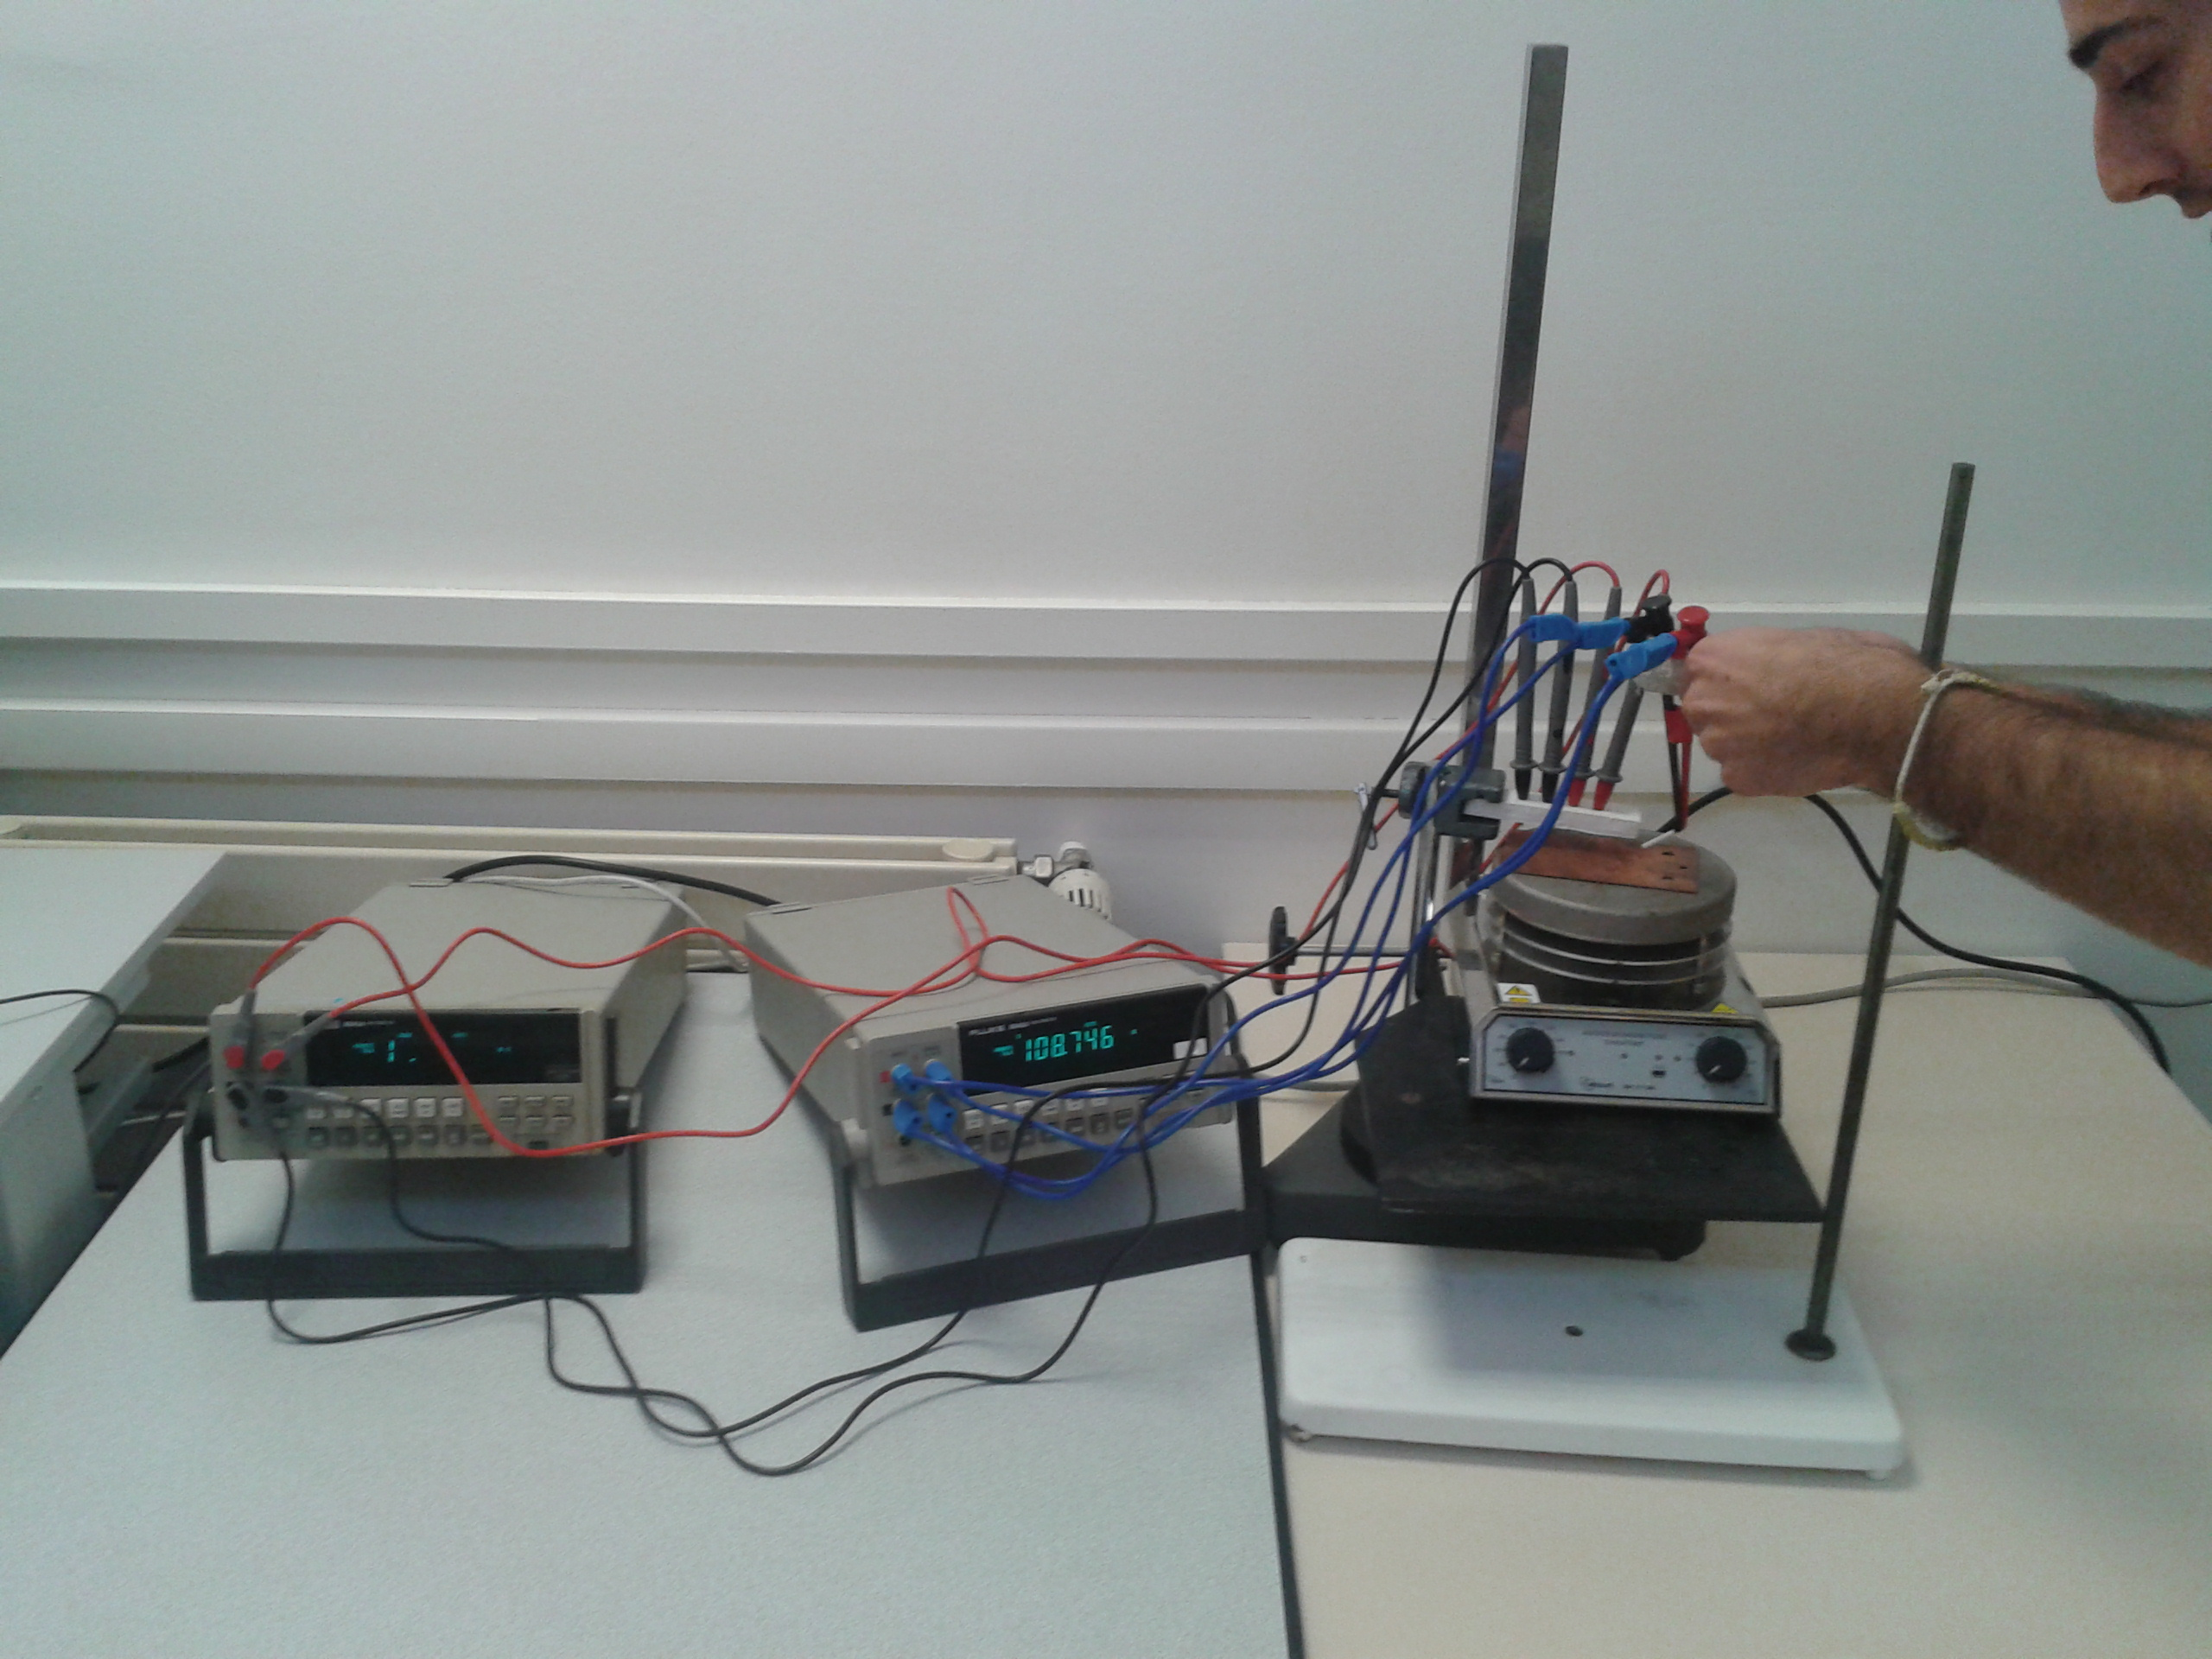
\includegraphics[width=12cm]{./images/photo1.jpg}
		\caption{Montage général}
		\label{photo1}
	\end{center}
\end{figure}

\newpage

\begin{figure}[!t]
  \begin{center}
		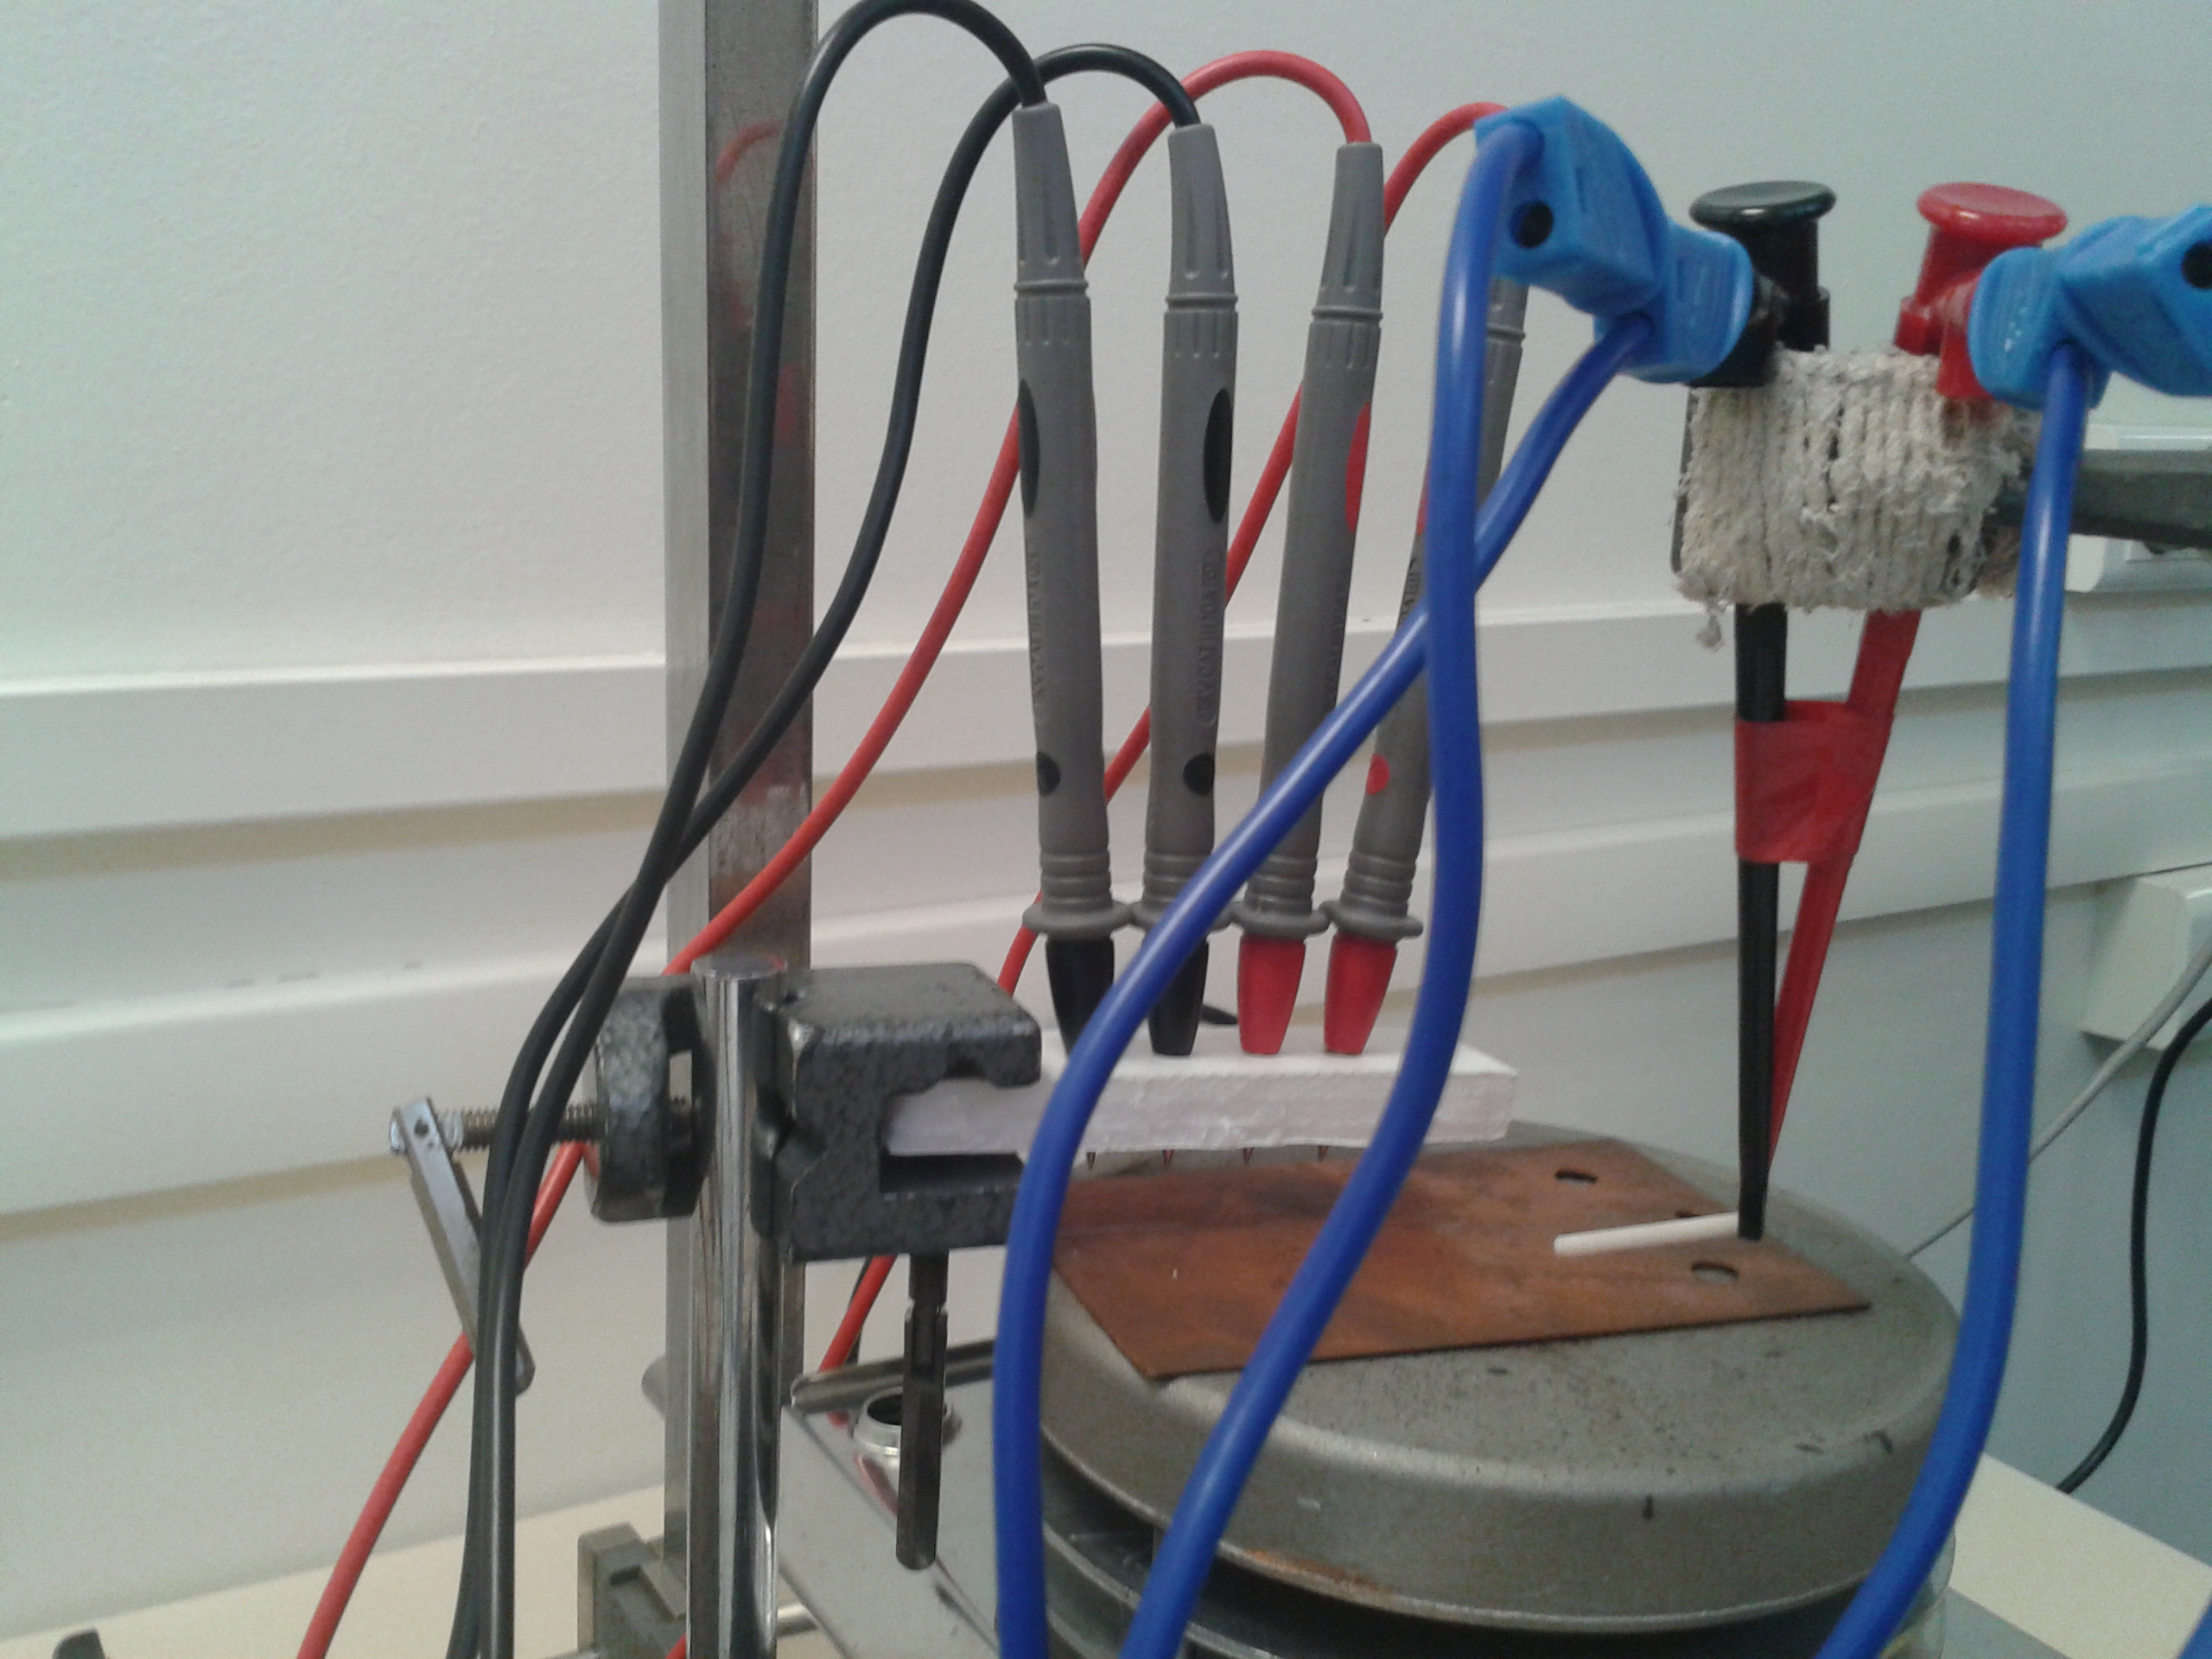
\includegraphics[width=8cm]{./images/photo2.jpg}
		\caption{Gros plan sur les 4 sondes de mesure de résistance (à gauche) et la sonde \emph{Pt100} de température (à droite)}
		\label{photo2}
	\end{center}
\end{figure}
\begin{figure}[h]
  \begin{center}
		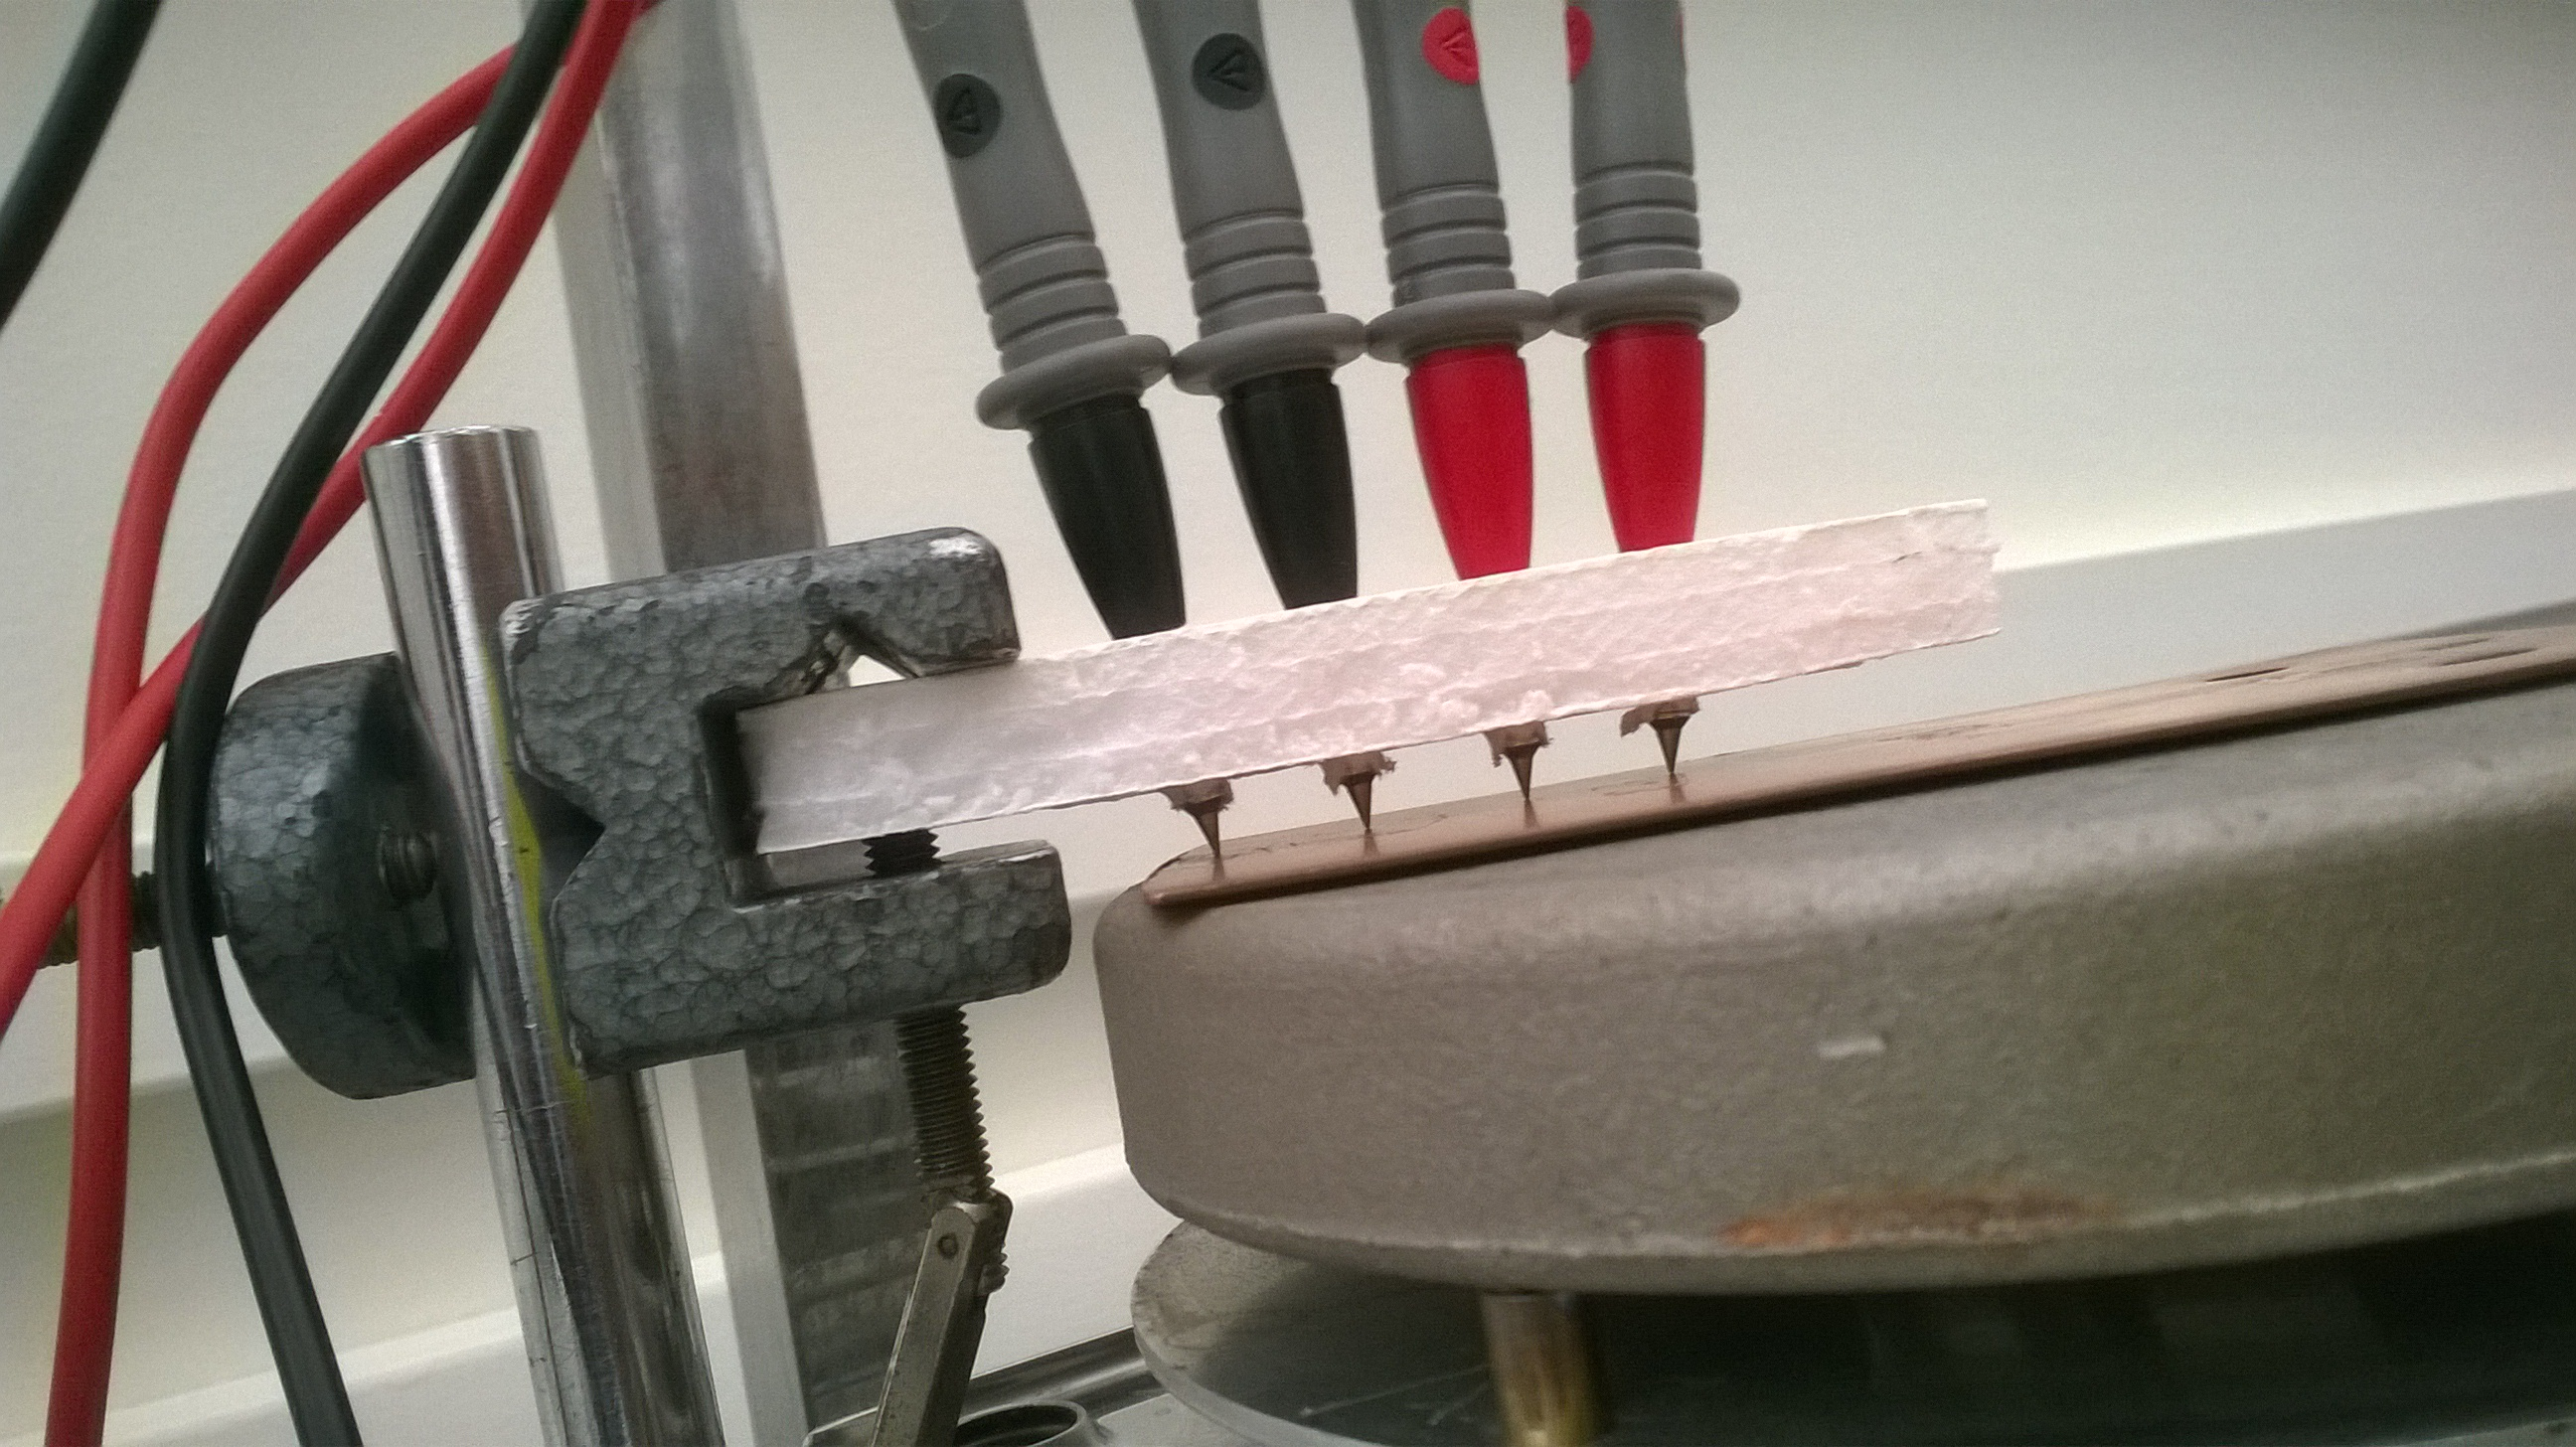
\includegraphics[width=9cm]{./images/photo3.jpg}
		\caption{Les 4 pointes en contact}
		\label{photo3}
	\end{center}
\end{figure}

Sur les 2 photos suivantes : Figures \ref{photo4} et \ref{photo5}, on peut voir le porte-échantillon rempli de billes 
de verre, et dans lequel est inséré la sonde de température (dans le but d'améliorer l'inertie thermique), ce montage étant utilisé dans le cas du refroidissement à l'azote liquide (on verse l'azote dans ce porte-échantillon adapté à ce type de manipulations à très basse température).

\newpage

\begin{figure}[!t]
  \begin{center}
		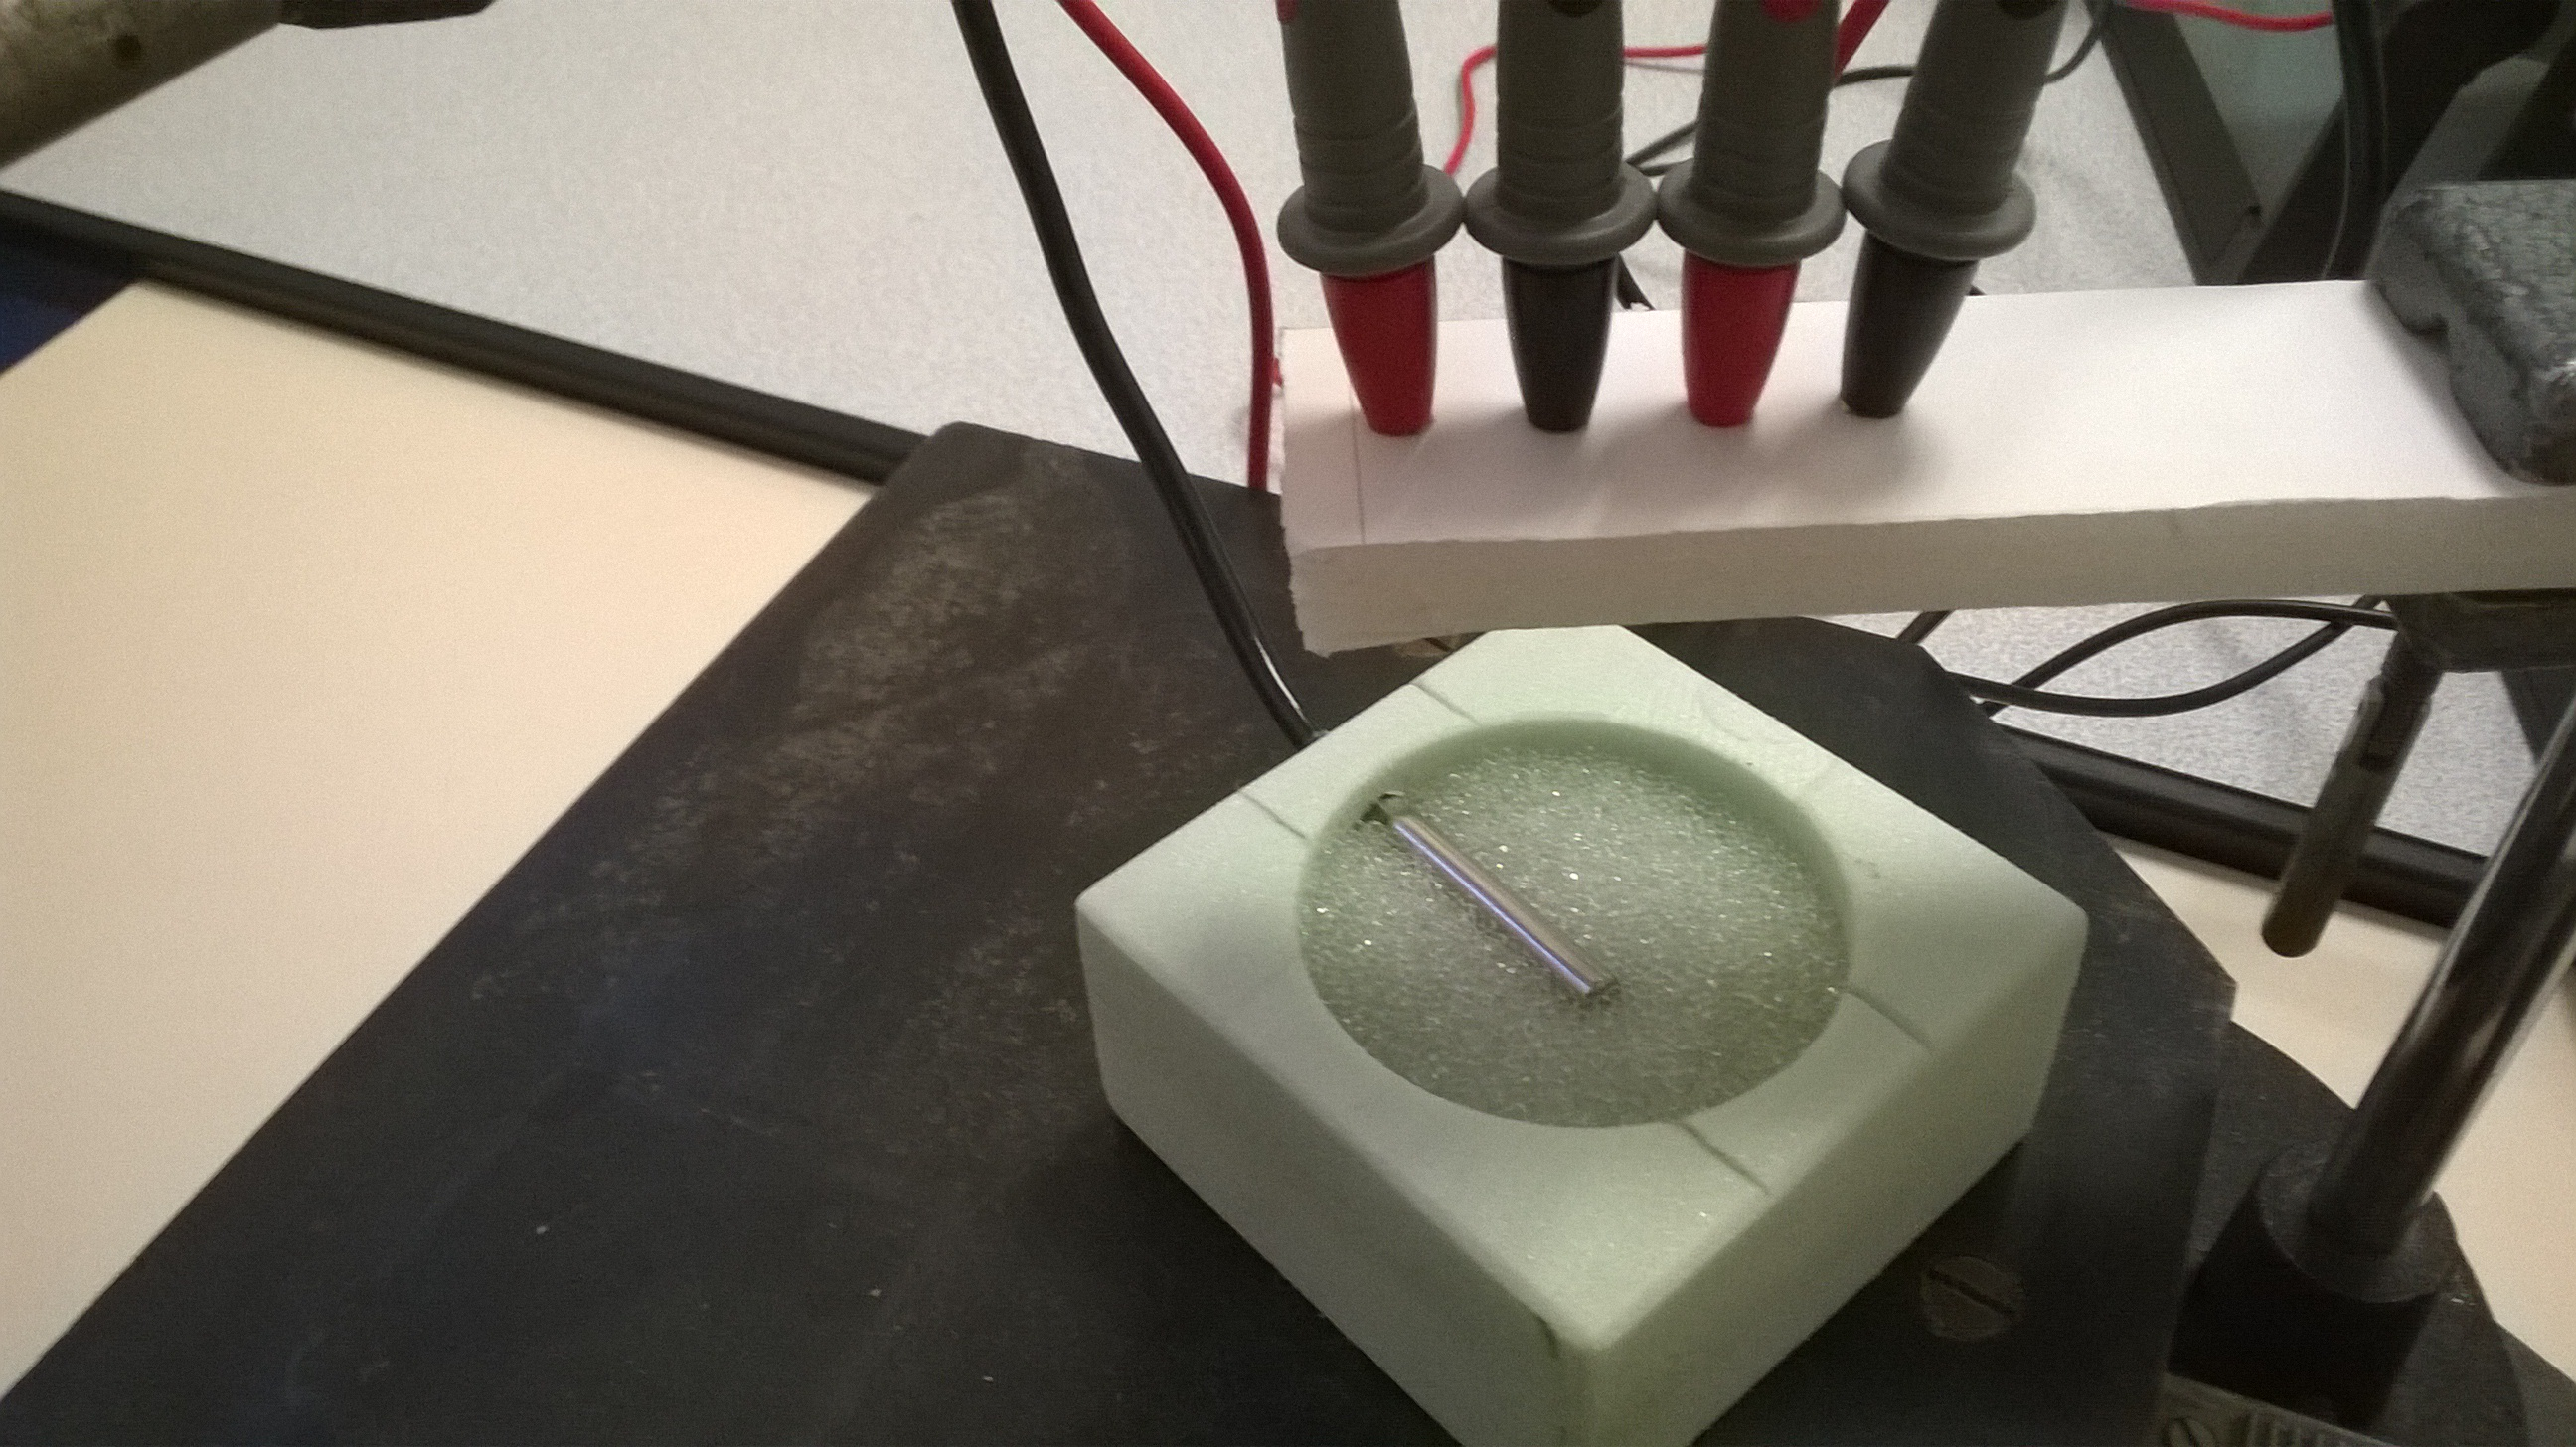
\includegraphics[width=7cm]{./images/photo4.jpg}
		\caption{Porte-échantillon pour le refroidissement à l'azote liquide avec une sonde de température insérée sur le côté.}
		\label{photo4}
	\end{center}
\end{figure}

\begin{figure}
  \begin{center}
		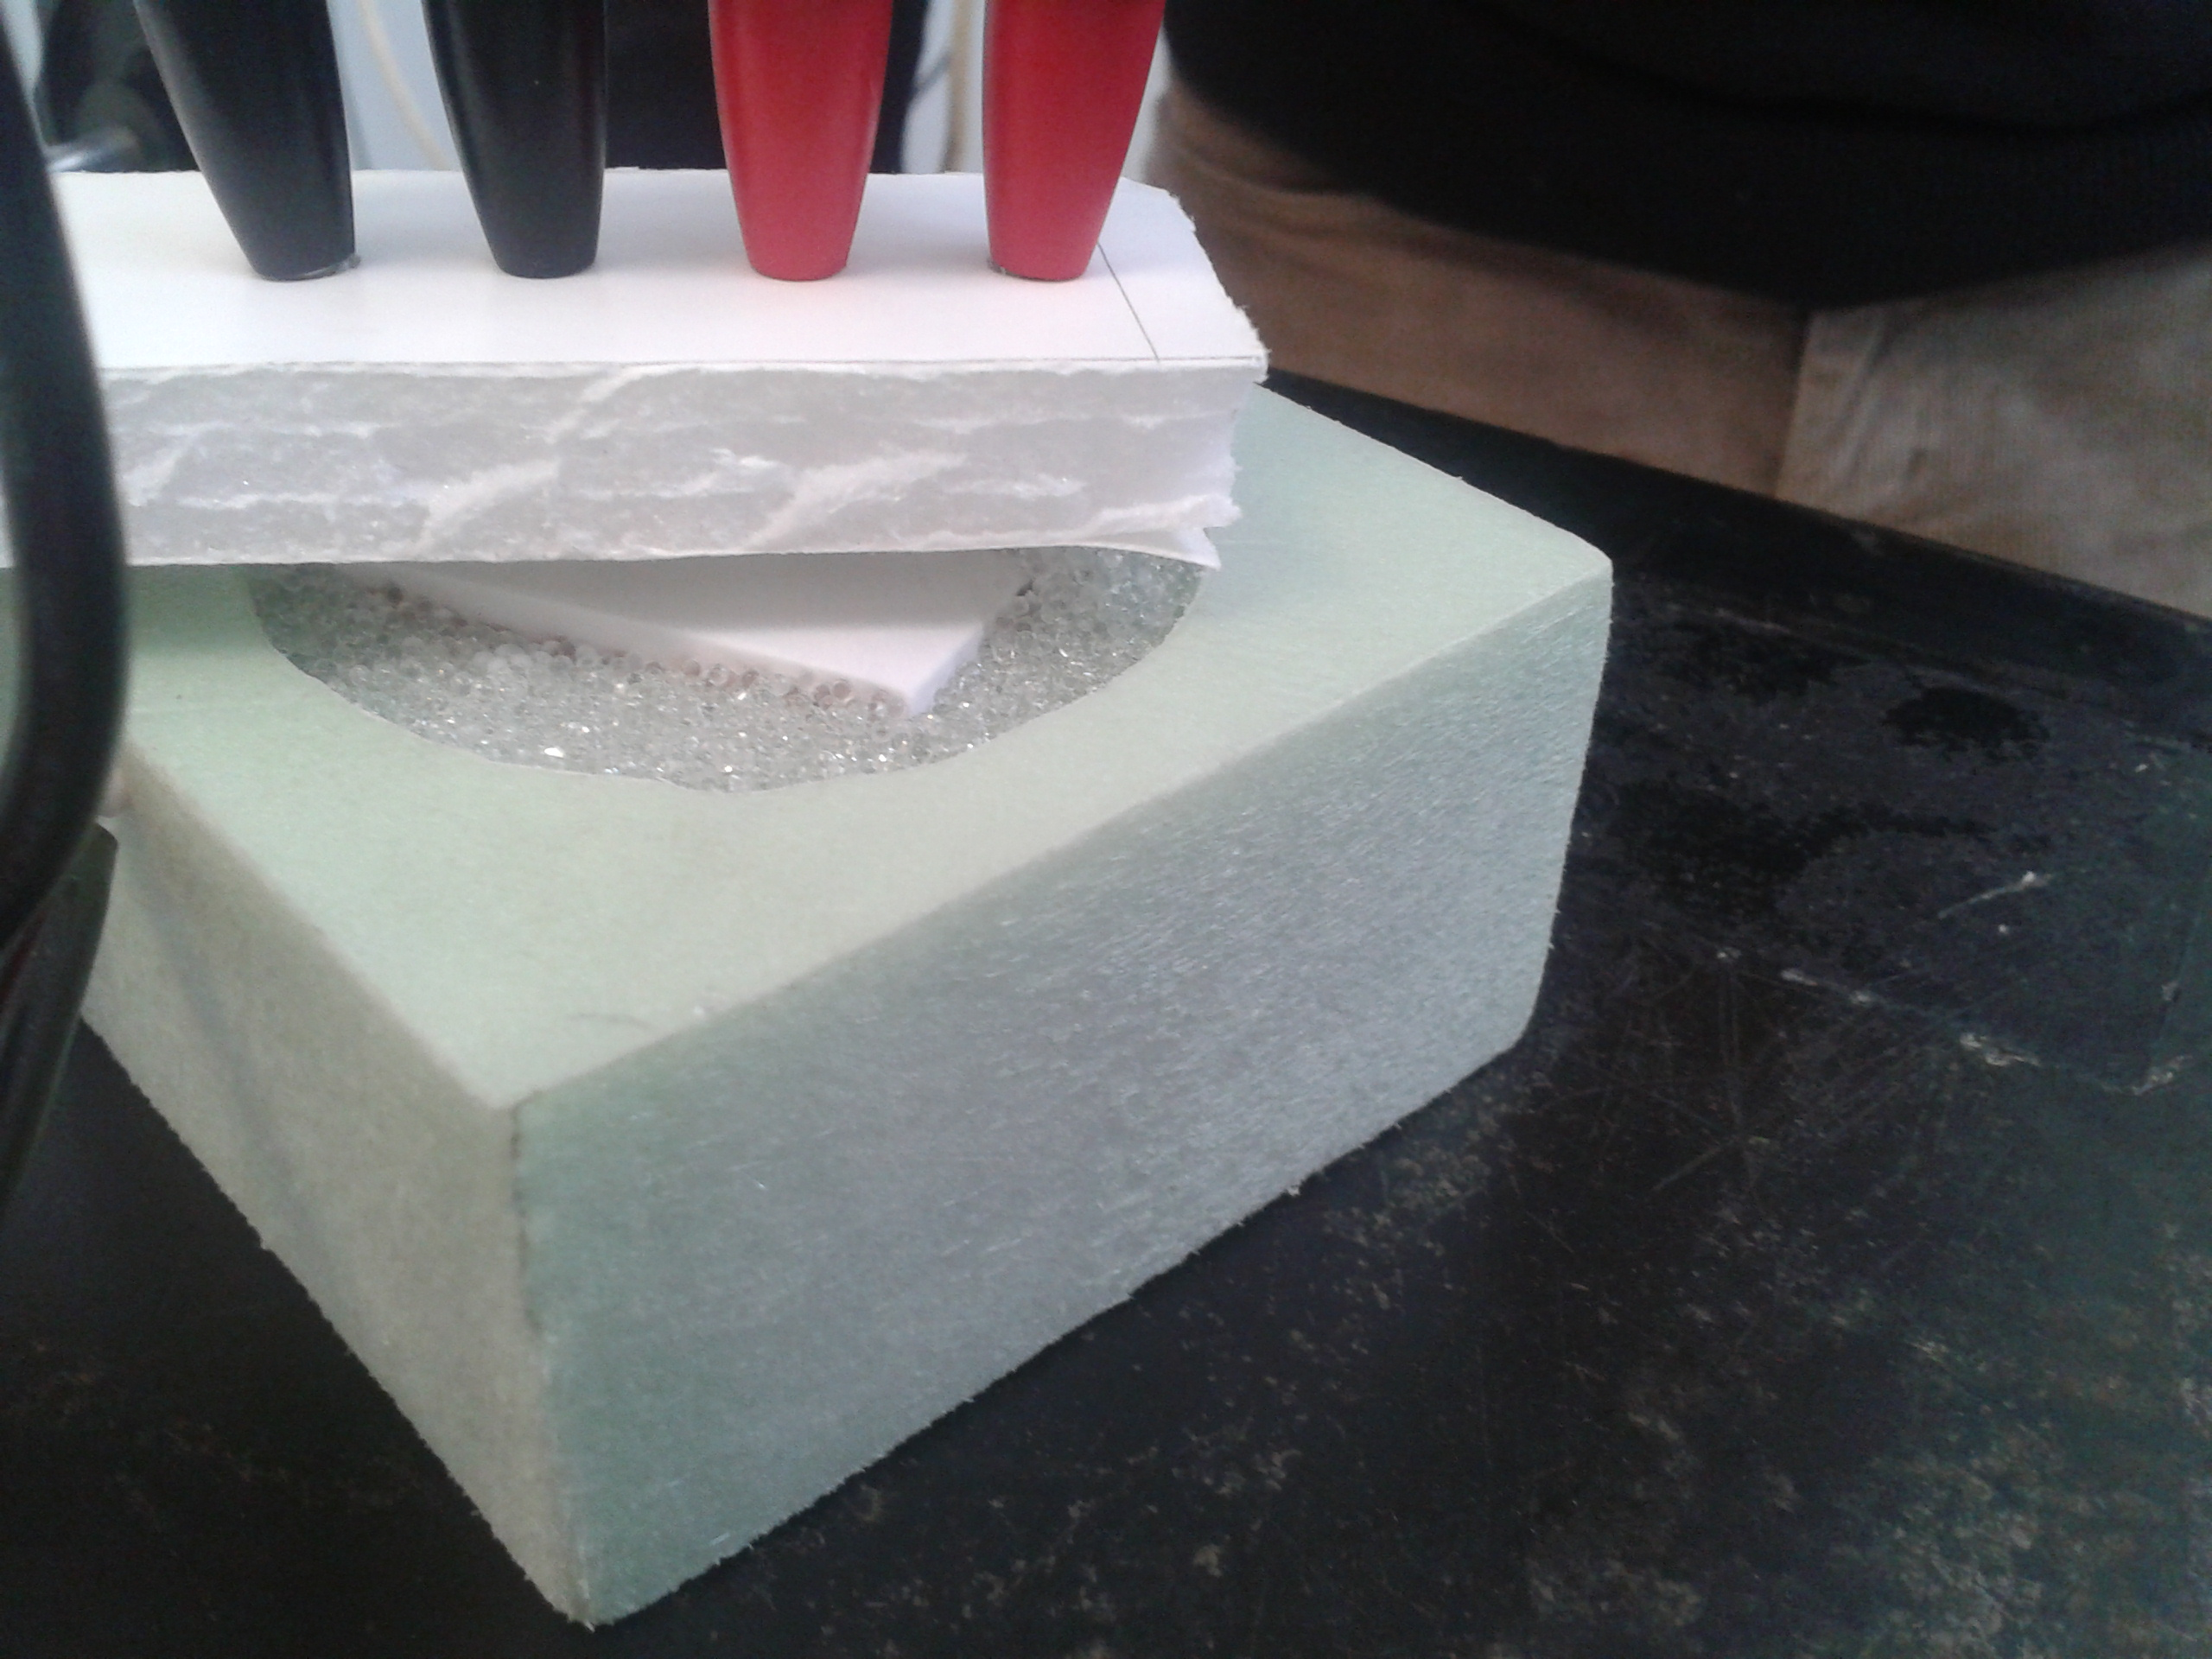
\includegraphics[width=7cm]{./images/photo5.jpg}
		\caption{Les 4 pointes en contact au cours d'une mesure avec refroidissement à l'azote liquide (ici, il s'agit d'un essai avec une petite plaque de cuivre).}
		\label{photo5}
	\end{center}
\end{figure}

Voici enfin une photo du montage à effet Hall [Figure \ref{photo_hall}], que nous avions commencé à préparé, 
mais que nous n'avons malheureusement pas eu le temps de terminer. Nous voulions utiliser un électroaimant, 
on peut aussi observer une source de courant sur la table, ainsi qu'une potence à gauche de l'électroaimant, destinée à maintenir l'échantillon.

\begin{figure}[!t]
  \begin{center}
		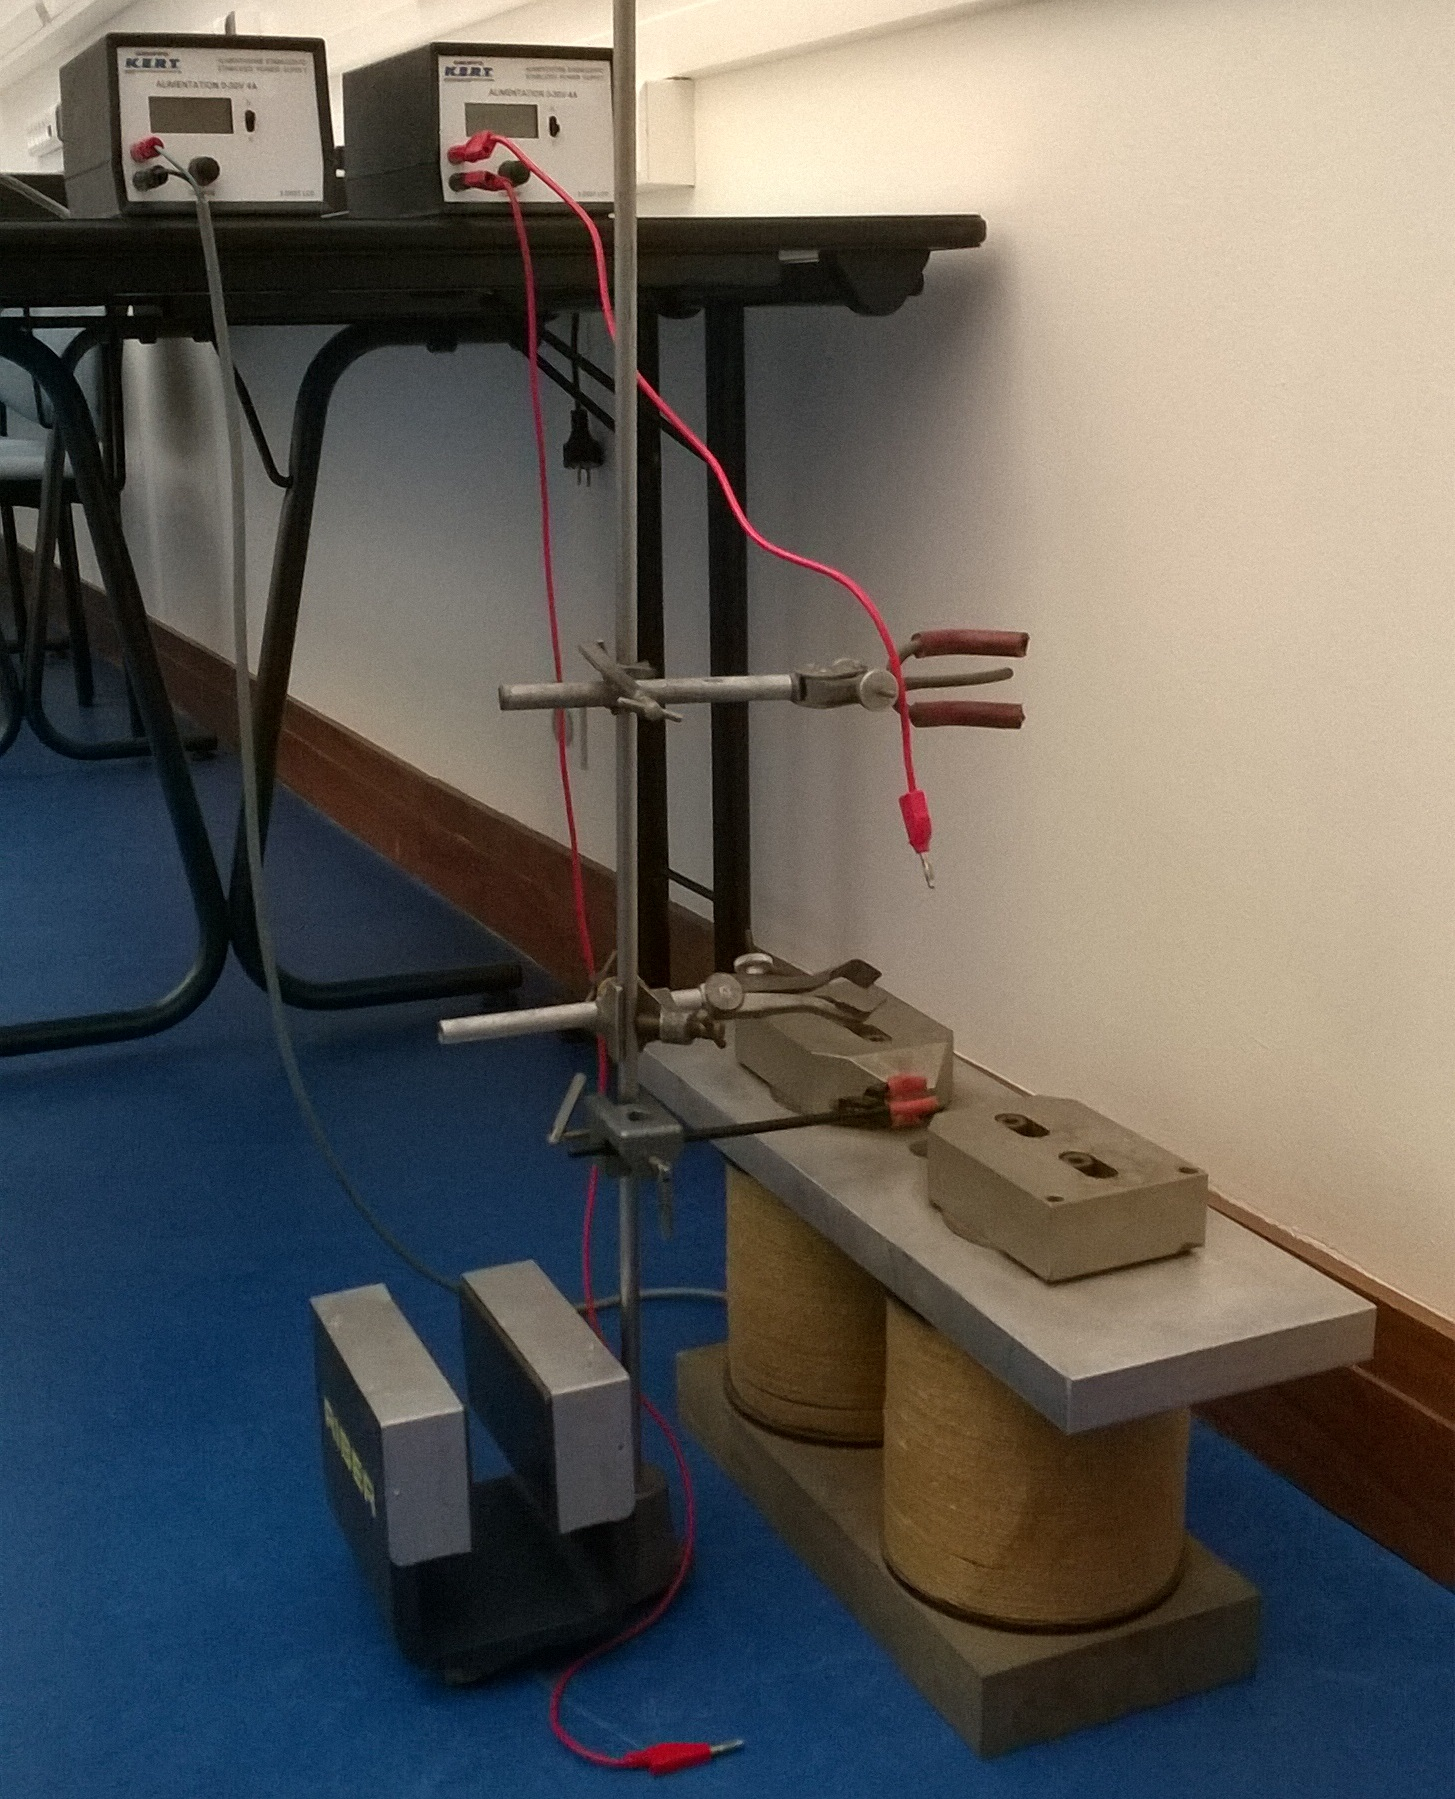
\includegraphics[height=6cm]{./images/photo_hall.jpg}
		\caption{Montage pour la mesure à effet Hall}
		\label{photo_hall}
	\end{center}
\end{figure}

\newpage

\subsection{Conditions expérimentales}
Nous avons utilisé Labview pour réaliser les acquisitions des deux résistances mesurées.
Nous avons simplement posé la plaque de cuivre sur une plaque chauffante et mesuré sa résistance en fonction de la température en 4 pointes, entre 25\celsius{} et 205\celsius{}.


Pour le silicium, nous voulions détecter un palier de conductivité (car il s'agissait d'échantillons dopés, cf. section \ref{objectifs}),
et nous savions que ce palier risquait de se trouver à une température inférieure ou égale à la température 
ambiante (voir \cite{kittel_introduction_1976}).
Donc, pour pouvoir étudier ce palier, nous avons dû baisser fortement la température et nous avons utilisé de l'azote liquide pour cela.
Nous avons également placé des billes de verre dans notre porte-échantillon pour augmenter l'inertie thermique du montage et nous permettre d'avoir une montée en température relativement lente.
La sonde de température a été insérée dans le porte-échantillon par un trou percé sur le côté (voir Figure \ref{photo4}). De cette façon, elle peut être en contact avec silicium et être entourée par les billes de verre.
De ce fait, elle mesure bien mieux la température du silicium que si on l'avait simplement posée sur l'échantillon,
où la thermalisation dûe à l'air aurait entraîné des biais.


\paragraph{Pourquoi une mesure 4 pointes (et pas tout simplement 2) ?}
La mesure 4 pointes consiste à injecter un courant avec deux pointes et à mesurer une tension avec deux 
autres placées entre les deux premières (cf. figure \ref{photo3}).
Cette méthode permet de s'affranchir des résistances des fils et des résistances de contact.
Elle est donc particulièrement utile pour mesurer des résistances de l'ordre de l'$\Omega$ ou inférieures, car c'est l'ordre de grandeur des résistances parasites.
Par contre, elle est peu utile pour les hautes résistances (plusieurs k$\Omega$, M$\Omega$), donc nous aurions mesuré en 2 pointes pour un isolant par exemple.


\paragraph{Principe et étalonnage de la sonde}
Nous avons étalonné la sonde Pt en deux étapes :

\begin{itemize}
  \item en la plaçant dans de l'eau que nous avons fait bouillir, nous avons pu mesurer la résistance de la sonde à une température de 100\celsius{}.
  \item en la plaçant ensuite dans de l'eau pleine de glaçons, nous avons fait la même chose pour 0\celsius{}.
\end{itemize}

La résistance du platine augmente linéairement avec la température, c'est une propriété de ce matériau.
On obtient alors la caratéristique R(T) : en mesurant la résistance du Platine, on peut en déduire sa température 
(donc idéalement la température de l'échantillon en contact avec la sonde).


\paragraph{Interfaçage grâce à Labview}
L'utilisation de l'outil informatique pour mener à bien l'expérience était prévu pour cet AE et en constituait une des principales caractéristiques. En effet notre encadrant nous avait fortement recommandé d'automatiser les mesures pour faciliter la prise de données tout en gagnant en savoir-faire expérimental. L'outil de prédilection pour ce type de mesure est le logiciel \emph{Labview} qui permet de réaliser l'acquisition et le traitement des données. Nous avons donc décidé d'utiliser ce logiciel. Le but était de pouvoir contrôler les deux multimètres avec l'ordinateur. La prise de données par voie informatique comporte trois volets que nous avons dû nous approprier successivement : 

\begin{enumerate}
\item la connexion des appareils à l'ordinateur, 
\item leur reconnaissance par ce dernier, 
\item et la réalisation du code Labview. 
\end{enumerate}

La première étape a été réalisée grâce à deux câbles \emph{smart488}, mais le laboratoire n'ayant qu'un seul câble 
de ce type, nous avons dû en commander en deuxième (cf. annexe \ref{annexe_factures}).
Ces câbles permettent le passage d'une sortie GPIB à une sortie USB et possèdent un contrôleur intégré. 
C'est ce contrôleur qu'il a fallu régler, grâce à un logiciel dédié, pour pouvoir détecter les deux multimètres 
via l'ordinateur. Nous avons aussi utilisé le logiciel NI-Max pour vérifier la compatibilité de ces éléments avec Labview. 

Après cela nous avons entamé l'étape d'écriture du code graphique Labview [Figure \ref{code_labview}]. Ce code devait nous permettre d'acquérir 
simultanément, et dans le temps, les signaux des deux multimètres, qui correspondent 
respectivement à la température de la sonde 
et à la résistance de l'échantillon. L'acquisition se fait pendant un laps de temps prédéfini. 
Les résultats obtenus sont présentés sous forme de tableau de nombres dans un fichier texte qui peut être 
lisible par un logiciel comme de traitement de données comme \textit{gnuplot} ou \textit{Excel}.
Nous avons en effet utilisé \textit{gnuplot} par la suite pour tracer nos courbes.

\begin{figure}[!t]
  \begin{center}
		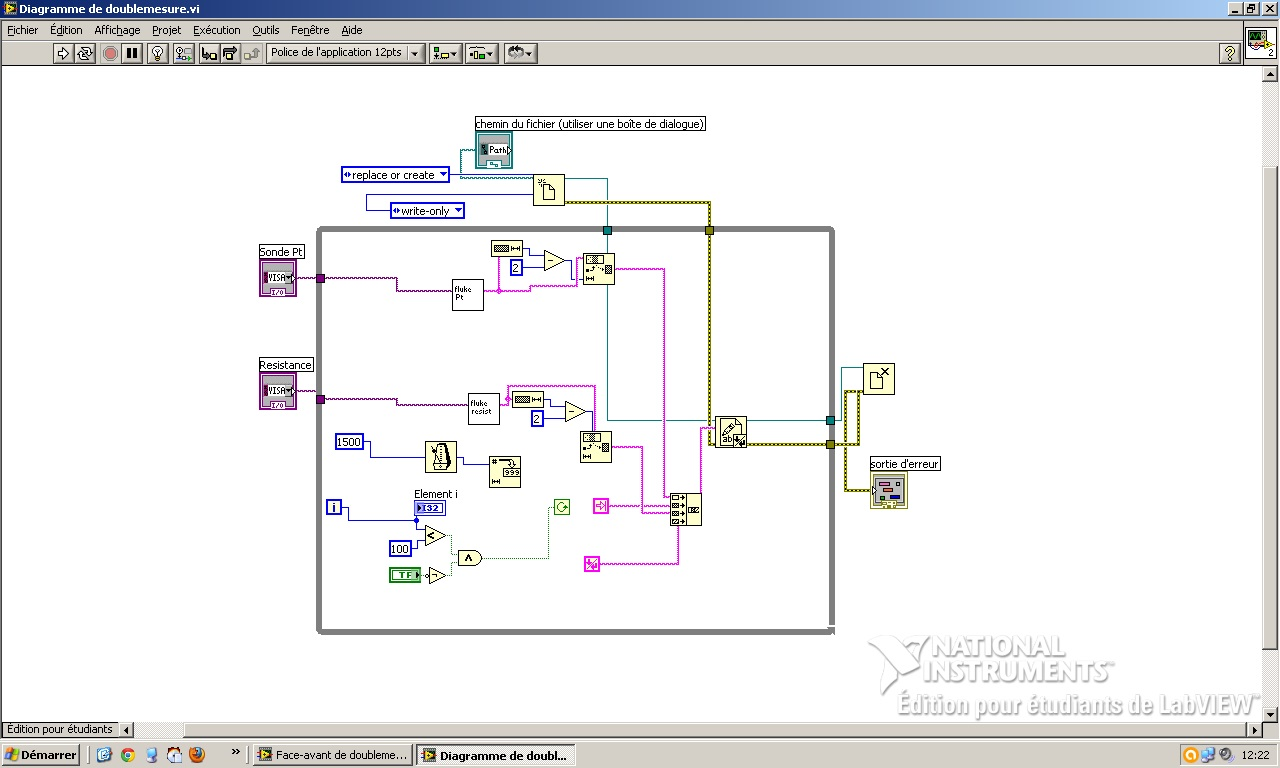
\includegraphics[height=6cm]{./images/labview.jpg}
		\caption{Code de notre programme Labview}
		\label{code_labview}
	\end{center}
\end{figure}

\newpage

\subsection{Difficultés expérimentales}
Deux principales difficultés expérimentales se sont posées lors de cette activité.
Tout d'abord, il y a eu le problème de l'automatisation des résultats et de l'interfaçage avec l'ordinateur.
Nous avons eu du mal à réaliser chacune des trois étapes liées à l'automatisation des mesures, 
mais plus particulièrement 
la détection des instruments par l'ordinateur, ceci mettant en jeu différents composants tels que le 
multimètre, le câble smart488 et Labview.

\bigskip

D'autre part, le contact entre les électrodes et l'échantillon s'avéra bien plus délicat que prévu. 
En effet l'utilisation du montage à quatre pointes oblige à avoir quatre contacts stables.

Nous avons d'abord utilisé de la laque d'argent pour réaliser les contacts, mais cela ne s'est pas avéré facile 
à mettre en place ni très efficace (en effet, à haute température, la laque d'argent ne tenait pas).
Nous avons donc implémenté le montage tel qu'il apparaît dans les photos [Figures \ref{photo1} à \ref{photo5}].

Le premier essai sur le cuivre donna des résultats 
très cohérents mais les essais sur les échantillons de silicium donnaient des valeurs très instables. 
En effet la valeur de la résistance changeait de plusieurs ordres de grandeurs selon la pression exercée sur les 
pointes.

\bigskip

Nous soupçonnons les fils et les pointes d'être a l'origine de ces fluctuations (contacts imparfaits), mais une piste intéressante est l'hétérogénéité de la surface de l'échantillon de silicium. 
En effet le silicium au contact de l'air s'oxyde et on obtient une couche de SiO$_2$ à la surface de l'échantillon. 
La variation de la résistance selon la pression exercée sur les pointes peut donc provenir du fait que la pointe 
traverse ou pas cette couche.

En effet, lorsque l'on exerce une pression constante on obtient des résultats cohérents avec la nature semiconductrice du silicium comme on pourra le voir dans la section suivante. Une façon d'obtenir cette pression constante et donc un meilleur contact est d'utiliser des pointes à ressorts, fixées solidement au support. Cependant, nous n'avons pas pu nous procurer de tels contacts avant la fin de l'activité et nous avons dû réaliser plusieurs fois la même expérience jusqu'à obtenir une mesure stable.

\subsection{Résultats}
Pour commencer et avant de s'attaquer à une mesure sur un semi-conducteur qui s'annonçait complexe, 
nous avons testé notre montage comme annoncé précédemment avec une mesure sur un conducteur très simple : 
une plaque de cuivre.

Nous avons posé la plaque de Cu sur une plaque chauffante, et nous avons mesuré sa résistance en 4 pointes pour 
des températures allant de la température ambiante (environ 20 \celsius{}) à environ 200 \celsius{}. La sonde Pt100 était posée sur la plaque pour suivre la température, comme on peut le voir sur la Figure \ref{photo2}. Toutes les mesures ont été prises via un interfaçage avec Labview.

\bigskip

Nous avons ainsi observé très logiquement une augmentation de la résistance de la plaque en fonction de la température. On peut observer cette tendance sur la Figure \ref{courbe_cuivre}, sur laquelle une régression linéaire a été effectuée et pour laquelle on obtient un bon coefficient de corrélation : $R > 0.99$.

\begin{figure}[hb]
  \begin{center}
		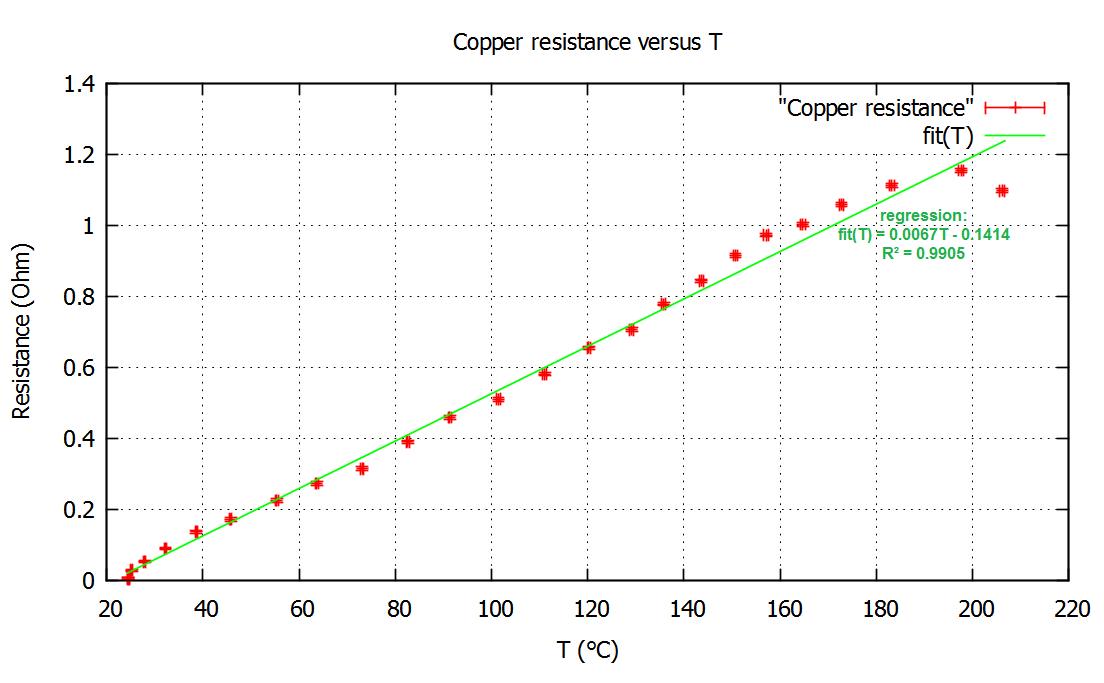
\includegraphics[width=12cm]{./images/Resistance_Cuivre_finale_english.png}
		\caption{Résistance de la plaque de cuivre en fonction de la température. En vert la régression linéaire et ses caractéristiques.}
		\label{courbe_cuivre}
	\end{center}
\end{figure}

\newpage

Ceci est bien en phase avec le modèle de Drude de la conduction électrique, pour lequel la conductivité d'un métal a cette expression (voir \cite{kittel_introduction_1976}) : 
\begin{equation}
	\sigma = \frac{n e^{2} \tau}{m}
\end{equation}
$n$ étant la densité volumique d'électrons, $e$ et $m$ la charge et la masse des électrons, et $\tau$ le temps de vol moyen entre deux collisions d'électrons. Plus la température augmente, plus le taux de collisions entre électrons augmente et donc plus $\tau$ diminue, ainsi $\sigma$ diminue et la résistance de l'échantillon augmente.

\bigskip

Ensuite, nous avons réalisé la mesure pour un wafer de silicium dopé de type N. Il a été placé sur un lit de billes de verre, billes dans lesquelles la sonde de température était placée (voir Figure \ref{photo4}). Là encore, la mesure a été effectuée en 4 pointes et avec l'aide de Labview une première fois (infructueuse), puis sans Labview pour pouvoir mieux contrôler le déroulement de la mesure. Les mesures ont donc été notées à la main. On peut observer les résultats sur la Figure \ref{courbe_silicium}.

\begin{figure}[hb]
  \begin{center}
		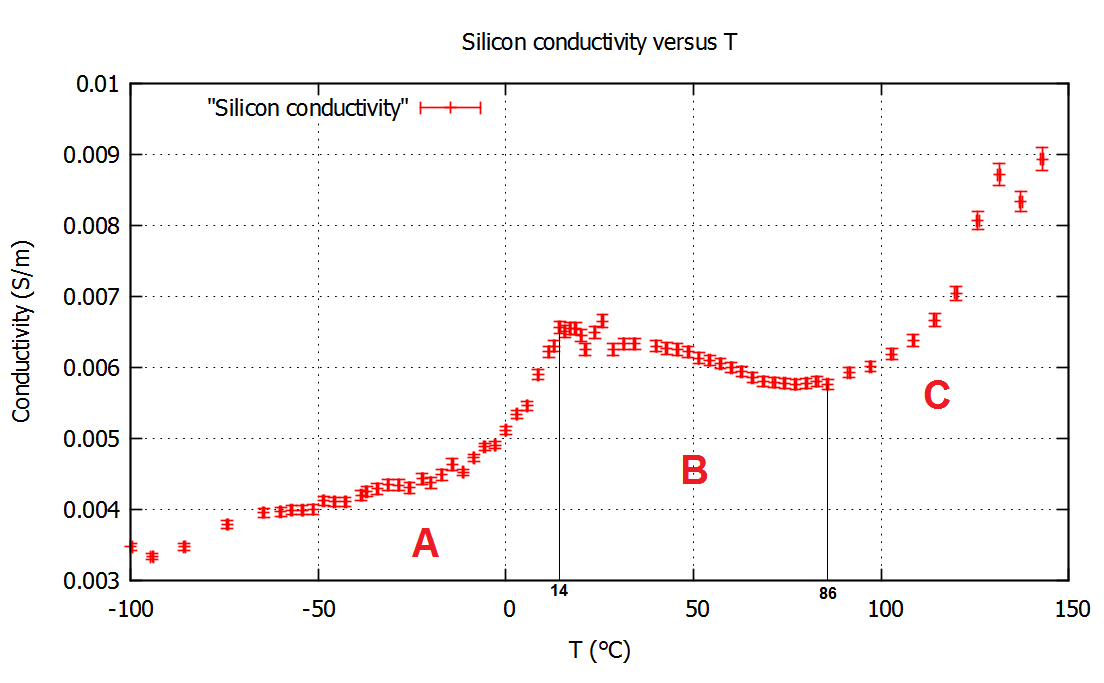
\includegraphics[width=12cm]{./images/Conductivite_Silicium_finale_english.png}
		\caption{Conductivité du wafer de silicium de type N en fonction de la température. Les trois régimes sont notés A, B et C. Le régime A est une croissance en loi d'Arrhénius pour les électrons venant des impuretés. Le régime B est un palier. Le régime C est lui aussi en loi d'Arrhénius, cette fois-ci pour les électrons venant de la bande de valence.}
		\label{courbe_silicium}
	\end{center}
\end{figure}

\newpage

Nous avons bien observé une conductivité croissante avec la température comme prévu, avec un palier aux alentours de [20\celsius{}; 80\celsius{}], ce qui est cohérent avec ce qu'on peut trouver dans \cite{kittel_introduction_1976}. On peut ainsi observer les trois régimes différents sur la Figure \ref{courbe_silicium}.

Le premier régime (A), allant d'environ -100 \celsius{} à 14 \celsius{}, suit une loi d'Arrhénius. 

Le second régime (B) est un palier allant d'environ 14 \celsius{} à 86 \celsius{}. La conductivité 
décroît faiblement dans cet intervalle de température. 

Le dernier régime (C) suit une loi d'Arrhénius entre 86 \celsius{} et 150 \celsius{} environ, comme le premier régime.


\paragraph{Remarques :}
Nous n'avons pas pu mesurer en-dessous de -100 \celsius{} environ car l'échantillon même baigné dans l'azote se réchauffait trop vite. De même, nous n'avons pas poursuivi la montée en température au delà de 200 \celsius{} car déjà entre 150 \celsius{} et 200 \celsius{} les contacts se sont dégradés et les mesures devenaient aberrantes.

\subsection{Discussion des résultats}
Pour bien interpréter ces résultats, revenons sur le principe de dopage. L'échantillon étudié
est dopé avec des atomes de phosphore, qui sont insérés dans l'échantillon de silicium intrinsèque. Ceci revient à introduire des niveaux d'énergie supplémentaires entre la bande de valence et la bande de conduction (voir Figure \ref{doping}).

\begin{figure}[ht]
  \begin{center}
		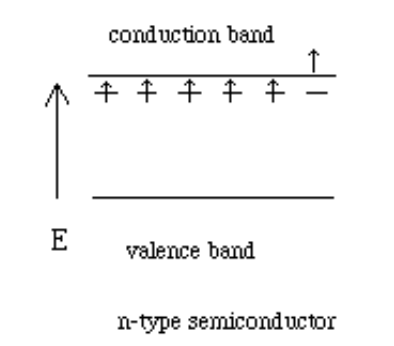
\includegraphics[width=5cm]{./images/doping.png}
		\caption{Les impuretés génèrent des niveaux d'énergie supplémentaires au sein de la bande interdite, ce qui nous amène à la configuration de cette figure.}
		\label{doping}
	\end{center}
\end{figure}

On peut ainsi expliciter les mécanismes qui nous amènent à observer ces trois régimes lorsqu'on augmente la température : 
\begin{description}
\item[Température très basse (non observé) : ] Pour de très basses températures, les fluctuations thermiques n'apportent pas assez d'énergie aux électrons pour qu'ils passent dans la bande de conduction, le matériau est donc \emph{isolant}.
\item[Régime A : ] Ensuite, au fur et à mesure que la température augmente, de plus en plus d'électrons venant des 
impuretés peuvent acquérir suffisamment d'énergie pour passer dans la bande de conduction et donc conduire le courant, 
le matériau devient donc \emph{conducteur}. Il est d'autant plus conducteur que la température est grande car de plus 
en plus d'électrons peuvent être promus dans la bande de conduction puisque l'énergie thermique qu'ils peuvent recevoir
augmente. On parle du \textbf{régime d'impuretés}.
\item[Régime B : ] Quand tous les électrons venant des impuretés sont passés dans la bande de conduction 
mais que l'énergie thermique n'est pas encore suffisante pour promouvoir les électrons de la bande de valence, 
il n'y a pas de nouvelle contribution à la conduction quelle que soit la température. Nous observons donc un palier, 
et même une légère diminution de la conductivité. En effet, comme dans un métal, le taux de collision entre électrons 
dans la bande de conduction augmente avec la température, ce qui diminue la conductivité. C'est le \textbf{régime de saturation}.
\item[Régime C : ] Enfin, quand l'énergie thermique est suffisante, les électrons de la bande de valence commencent à 
passer dans la bande de conduction comme dans le cas du régime A avec les impuretés. On a donc une seconde phase de 
croissance. Il s'agit du \textbf{régime intrinsèque}.
\end{description}

Les deux phases de croissance observées (A et C) suivent une loi d'Arrhénius, c'est-à-dire une loi faisant intervenir une probabilité de transition (vers la bande de conduction en l'occurence) dépendant d'une énergie d'activation (ici la moitié de l'énergie du "gap" entre les bandes considérées). On a donc une densité $n$ d'électrons dans la bande de conduction de la forme : 
\begin{equation}
	n \propto exp \left( - \frac{\Delta E}{2 k_{B} T} \right)
\end{equation}
où $\Delta E$ représente la différence d'énergie entre la bande de conduction et les niveaux d'énergie des impuretés si on considère la densité d'électrons venant des impuretés ; ou bien la différence d'énergie entre la bande de conduction et la bande de valence si on prend en compte la densité d'électrons venant de cette dernière.

Puisque la conductivité du semi-conducteur est proportionnelle à la densité d'électrons dans la bande de conduction, on obtient bien deux lois d'Arrhénius pour la conductivité tantôt pour les électrons venant des impuretés, puis pour ceux venant de la bande de valence.

Pour vérifier que ces courbes montrent bien deux croissances suivant une loi d'Arrhénius, nous avons tracé le logarithme de la conductivité en fonction de $-\frac{1}{T}$, courbe qui devrait être une droite. Nous avons donc effectué deux régressions linéaires sur les deux zones de croissance (voir Figure \ref{log}).

Nous avons éliminé certains points pour ces régressions, notamment les points à basse température qui ne semblaient 
pas faire partie de la zone de croissance du régime A. À partir de ces régressions, nous avons pu estimer les énergies 
d'activation et donc les gaps $\Delta E$. Le gap entre la bande de conduction et les niveaux d'énergie des impuretés 
est d'environ $\Delta E = 0.2 eV$, et le gap entre les bandes de valence et de conduction est d'environ $\Delta E = 0.7 eV$. 
Cette valeur est tout à fait du bon ordre de grandeur pour du silicium (voir \cite{kittel_introduction_1976}), et le 
gap concernant les impuretés est $3.5$ fois plus faible, ce qui paraît cohérent avec le fait que les impuretés introduisent 
des niveaux d'énergie au sein de la bande interdite, donc d'énergie supérieure à celle des électrons de la bande de valence.

\begin{figure}[ht]
  \begin{center}
		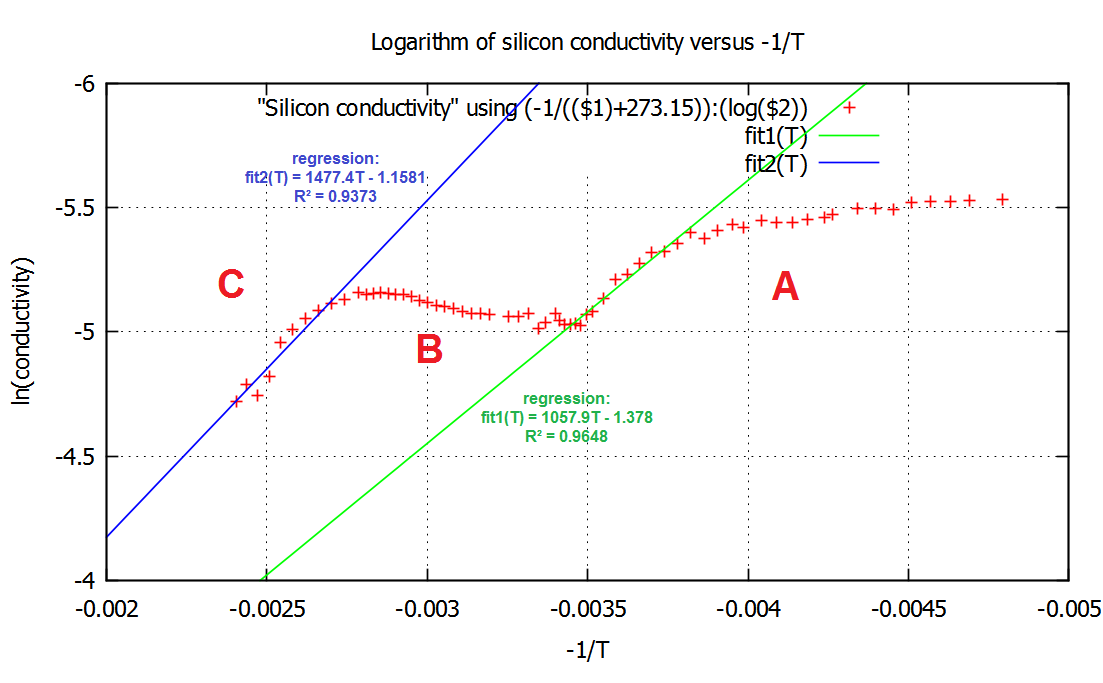
\includegraphics[width=11cm]{./images/Fit_de_log(sigma)_versus_-inverse(T).png}
		\caption{Tracé de log($\sigma$) en fonction de $-\frac{1}{T}$. Deux régressions linéaires ont été effectuées sur les deux zones de croissance en loi d'Arrhénius.}
		\label{log}
	\end{center}
\end{figure}

\subsection{Conclusions}
Nous avons bien trouvé une allure de conductivité singulière pour notre échantillon de silicium dopé N. Nous avons 
dégagé trois régimes décrivant cette allure, qui sont tout à fait cohérents avec les phénomènes physiques en jeu. 
Nous avons ainsi pu déterminer un palier de conductivité entre la température ambiante et 80 \celsius{} environ.


\section{{Perspectives}}
Malgré les difficultés liées au montage expérimental, les manipulations ont assez bien fonctionné et les résultats obtenus sont cohérents.
Avec plus de temps, il aurait sans doute été possible de réaliser plus de mesures, avec différents types de semi-conducteurs, différents types de dopage, ou encore des isolants.
Bien entendu, nous aurions également souhaité effectuer le montage Hall pour pouvoir compléter la mesure de conductivité.
Enfin, nous aurions aussi pu raffiner notre code Labview et mieux interfacer la mesure avec celui-ci, rendant ainsi la manipulation plus aisée.


\appendix

\section{{Annexe sécurité}}
La sécurité est un sujet primordial dans tous les laboratoires et tout travail comportant des risques se doit d'être encadré par des règles strictes. Notre activité expérimentale comportait différentes manipulations à risque que nous avons identifiées : 

\begin{itemize}
  \item Manipulation de l'azote liquide.
  \item Manipulation de la plaque chauffante.
  \item Manipulation d'instruments à haute tension.
  \item Manipulation de la perceuse.
\end{itemize}

\bigskip
Pour chacun de ces aspects nous avons pris les précautions nécessaires pour minimiser les risques d'accidents.

Dans cette annexe, nous allons particulièrement nous intéresser aux précautions à prendre avec l'azote liquide (les autres instruments que nous avons utilisés sont beaucoup plus communs).

L'azote liquide est utilisé dans divers domaines de l'industrie et de la recherche. Nous l'avons utilisé pour pouvoir refroidir notre échantillon à très basse température. En effet la température de l’azote liquide (point d’ébullition à la pression atmosphérique) est de -196\celsius{}. 
Il existe plusieurs types de dangers reliés à la manipulation de l'azote liquide. Nous allons les présenter individuellement, accompagnés des mesures de sécurité à respecter.

\subsection{Très basse température}

\paragraph{Dangers}

\begin{itemize}
  \item Lorsque le liquide cryogénique entre en contact avec la peau, il peut provoquer des 
brûlures par le froid appelées gélures. Des gélures sur une grande surface de la peau peuvent être mortelles. 
  \item Les très basses températures diminuent la résilience et la ductilité de certains 
matériaux, qui se fragilisent et peuvent se briser facilement. Ceci peut se traduire par des coupures ou par un renversement d'un produit dangereux.
  \item Lors de la manipulation de l'azote liquide, l’air peut se condenser. Le condensat riche en oxygène augmente le risque d'incendie 
\end{itemize}

\paragraph{Mesures de sécurité}

\begin{itemize}
  \item Lors de toute manipulation de l'azote liquide il faut utiliser des gants appropriés, des vêtements couvrant tout le corps, des lunettes de sécurité et des chaussures fermées.
  \item Le transport du liquide doit être réalisé dans des récipients adaptés, résistants aux basses températures et aux chocs. Lors du déplacement du récipient il faut éviter tout choc ou mouvement risquant le renversement du liquide. Le sol des pièces contenant l'azote liquide doit être non inflammable.
\end{itemize}

\subsection{Pression}

\paragraph{Dangers}

L'azote liquide peut s'évaporer très rapidement et ainsi entraîner de grandes augmentations de volume, ceci pouvant se traduire par des explosions.
\paragraph{Mesures de sécurité}

Le transport se fait en utilisant un dewar avec un couvercle perméable qui puisse permette l'échappement du gaz. Le récipient principal doit contenir des valves permettant l'échappement du gaz lors de surpressions.

\subsection{Hypoxie}

\paragraph{Dangers}

Point relié au précédent : lors de l'évaporation, de l'azote liquide peut déplacer l'air contenu dans la salle et provoquer un manque d'oxygène appelé hypoxie. Lorsque le taux d'oxygène dans l'air passe en dessous de 17\% il y a un risque d'évanouissement. De plus le corps n'arrive pas à détecter le manque d'oxygène et il est donc très difficile de réagir avant l'évanouissement.
\paragraph{Mesures de sécurité}

Il faut travailler dans une zone aérée, surtout dans la salle où se trouve le récipient principal. Il ne faut pas manipuler l'azote liquide seul.






\bibliographystyle{plain}
\bibliography{parts/bibliography}

\end{document}
